% Options for packages loaded elsewhere
\PassOptionsToPackage{unicode}{hyperref}
\PassOptionsToPackage{hyphens}{url}
%
\documentclass[
  a4paper,
]{book}

\usepackage{amsmath,amssymb}
\usepackage{iftex}
\ifPDFTeX
  \usepackage[T1]{fontenc}
  \usepackage[utf8]{inputenc}
  \usepackage{textcomp} % provide euro and other symbols
\else % if luatex or xetex
  \usepackage{unicode-math}
  \defaultfontfeatures{Scale=MatchLowercase}
  \defaultfontfeatures[\rmfamily]{Ligatures=TeX,Scale=1}
\fi
\usepackage{lmodern}
\ifPDFTeX\else  
    % xetex/luatex font selection
    \setmainfont[]{TH Sarabun New}
\fi
% Use upquote if available, for straight quotes in verbatim environments
\IfFileExists{upquote.sty}{\usepackage{upquote}}{}
\IfFileExists{microtype.sty}{% use microtype if available
  \usepackage[]{microtype}
  \UseMicrotypeSet[protrusion]{basicmath} % disable protrusion for tt fonts
}{}
\makeatletter
\@ifundefined{KOMAClassName}{% if non-KOMA class
  \IfFileExists{parskip.sty}{%
    \usepackage{parskip}
  }{% else
    \setlength{\parindent}{0pt}
    \setlength{\parskip}{6pt plus 2pt minus 1pt}}
}{% if KOMA class
  \KOMAoptions{parskip=half}}
\makeatother
\usepackage{xcolor}
\setlength{\emergencystretch}{3em} % prevent overfull lines
\setcounter{secnumdepth}{5}
% Make \paragraph and \subparagraph free-standing
\makeatletter
\ifx\paragraph\undefined\else
  \let\oldparagraph\paragraph
  \renewcommand{\paragraph}{
    \@ifstar
      \xxxParagraphStar
      \xxxParagraphNoStar
  }
  \newcommand{\xxxParagraphStar}[1]{\oldparagraph*{#1}\mbox{}}
  \newcommand{\xxxParagraphNoStar}[1]{\oldparagraph{#1}\mbox{}}
\fi
\ifx\subparagraph\undefined\else
  \let\oldsubparagraph\subparagraph
  \renewcommand{\subparagraph}{
    \@ifstar
      \xxxSubParagraphStar
      \xxxSubParagraphNoStar
  }
  \newcommand{\xxxSubParagraphStar}[1]{\oldsubparagraph*{#1}\mbox{}}
  \newcommand{\xxxSubParagraphNoStar}[1]{\oldsubparagraph{#1}\mbox{}}
\fi
\makeatother

\usepackage{color}
\usepackage{fancyvrb}
\newcommand{\VerbBar}{|}
\newcommand{\VERB}{\Verb[commandchars=\\\{\}]}
\DefineVerbatimEnvironment{Highlighting}{Verbatim}{commandchars=\\\{\}}
% Add ',fontsize=\small' for more characters per line
\usepackage{framed}
\definecolor{shadecolor}{RGB}{241,243,245}
\newenvironment{Shaded}{\begin{snugshade}}{\end{snugshade}}
\newcommand{\AlertTok}[1]{\textcolor[rgb]{0.68,0.00,0.00}{#1}}
\newcommand{\AnnotationTok}[1]{\textcolor[rgb]{0.37,0.37,0.37}{#1}}
\newcommand{\AttributeTok}[1]{\textcolor[rgb]{0.40,0.45,0.13}{#1}}
\newcommand{\BaseNTok}[1]{\textcolor[rgb]{0.68,0.00,0.00}{#1}}
\newcommand{\BuiltInTok}[1]{\textcolor[rgb]{0.00,0.23,0.31}{#1}}
\newcommand{\CharTok}[1]{\textcolor[rgb]{0.13,0.47,0.30}{#1}}
\newcommand{\CommentTok}[1]{\textcolor[rgb]{0.37,0.37,0.37}{#1}}
\newcommand{\CommentVarTok}[1]{\textcolor[rgb]{0.37,0.37,0.37}{\textit{#1}}}
\newcommand{\ConstantTok}[1]{\textcolor[rgb]{0.56,0.35,0.01}{#1}}
\newcommand{\ControlFlowTok}[1]{\textcolor[rgb]{0.00,0.23,0.31}{\textbf{#1}}}
\newcommand{\DataTypeTok}[1]{\textcolor[rgb]{0.68,0.00,0.00}{#1}}
\newcommand{\DecValTok}[1]{\textcolor[rgb]{0.68,0.00,0.00}{#1}}
\newcommand{\DocumentationTok}[1]{\textcolor[rgb]{0.37,0.37,0.37}{\textit{#1}}}
\newcommand{\ErrorTok}[1]{\textcolor[rgb]{0.68,0.00,0.00}{#1}}
\newcommand{\ExtensionTok}[1]{\textcolor[rgb]{0.00,0.23,0.31}{#1}}
\newcommand{\FloatTok}[1]{\textcolor[rgb]{0.68,0.00,0.00}{#1}}
\newcommand{\FunctionTok}[1]{\textcolor[rgb]{0.28,0.35,0.67}{#1}}
\newcommand{\ImportTok}[1]{\textcolor[rgb]{0.00,0.46,0.62}{#1}}
\newcommand{\InformationTok}[1]{\textcolor[rgb]{0.37,0.37,0.37}{#1}}
\newcommand{\KeywordTok}[1]{\textcolor[rgb]{0.00,0.23,0.31}{\textbf{#1}}}
\newcommand{\NormalTok}[1]{\textcolor[rgb]{0.00,0.23,0.31}{#1}}
\newcommand{\OperatorTok}[1]{\textcolor[rgb]{0.37,0.37,0.37}{#1}}
\newcommand{\OtherTok}[1]{\textcolor[rgb]{0.00,0.23,0.31}{#1}}
\newcommand{\PreprocessorTok}[1]{\textcolor[rgb]{0.68,0.00,0.00}{#1}}
\newcommand{\RegionMarkerTok}[1]{\textcolor[rgb]{0.00,0.23,0.31}{#1}}
\newcommand{\SpecialCharTok}[1]{\textcolor[rgb]{0.37,0.37,0.37}{#1}}
\newcommand{\SpecialStringTok}[1]{\textcolor[rgb]{0.13,0.47,0.30}{#1}}
\newcommand{\StringTok}[1]{\textcolor[rgb]{0.13,0.47,0.30}{#1}}
\newcommand{\VariableTok}[1]{\textcolor[rgb]{0.07,0.07,0.07}{#1}}
\newcommand{\VerbatimStringTok}[1]{\textcolor[rgb]{0.13,0.47,0.30}{#1}}
\newcommand{\WarningTok}[1]{\textcolor[rgb]{0.37,0.37,0.37}{\textit{#1}}}

\providecommand{\tightlist}{%
  \setlength{\itemsep}{0pt}\setlength{\parskip}{0pt}}\usepackage{longtable,booktabs,array}
\usepackage{calc} % for calculating minipage widths
% Correct order of tables after \paragraph or \subparagraph
\usepackage{etoolbox}
\makeatletter
\patchcmd\longtable{\par}{\if@noskipsec\mbox{}\fi\par}{}{}
\makeatother
% Allow footnotes in longtable head/foot
\IfFileExists{footnotehyper.sty}{\usepackage{footnotehyper}}{\usepackage{footnote}}
\makesavenoteenv{longtable}
\usepackage{graphicx}
\makeatletter
\def\maxwidth{\ifdim\Gin@nat@width>\linewidth\linewidth\else\Gin@nat@width\fi}
\def\maxheight{\ifdim\Gin@nat@height>\textheight\textheight\else\Gin@nat@height\fi}
\makeatother
% Scale images if necessary, so that they will not overflow the page
% margins by default, and it is still possible to overwrite the defaults
% using explicit options in \includegraphics[width, height, ...]{}
\setkeys{Gin}{width=\maxwidth,height=\maxheight,keepaspectratio}
% Set default figure placement to htbp
\makeatletter
\def\fps@figure{htbp}
\makeatother
% definitions for citeproc citations
\NewDocumentCommand\citeproctext{}{}
\NewDocumentCommand\citeproc{mm}{%
  \begingroup\def\citeproctext{#2}\cite{#1}\endgroup}
\makeatletter
 % allow citations to break across lines
 \let\@cite@ofmt\@firstofone
 % avoid brackets around text for \cite:
 \def\@biblabel#1{}
 \def\@cite#1#2{{#1\if@tempswa , #2\fi}}
\makeatother
\newlength{\cslhangindent}
\setlength{\cslhangindent}{1.5em}
\newlength{\csllabelwidth}
\setlength{\csllabelwidth}{3em}
\newenvironment{CSLReferences}[2] % #1 hanging-indent, #2 entry-spacing
 {\begin{list}{}{%
  \setlength{\itemindent}{0pt}
  \setlength{\leftmargin}{0pt}
  \setlength{\parsep}{0pt}
  % turn on hanging indent if param 1 is 1
  \ifodd #1
   \setlength{\leftmargin}{\cslhangindent}
   \setlength{\itemindent}{-1\cslhangindent}
  \fi
  % set entry spacing
  \setlength{\itemsep}{#2\baselineskip}}}
 {\end{list}}
\usepackage{calc}
\newcommand{\CSLBlock}[1]{\hfill\break\parbox[t]{\linewidth}{\strut\ignorespaces#1\strut}}
\newcommand{\CSLLeftMargin}[1]{\parbox[t]{\csllabelwidth}{\strut#1\strut}}
\newcommand{\CSLRightInline}[1]{\parbox[t]{\linewidth - \csllabelwidth}{\strut#1\strut}}
\newcommand{\CSLIndent}[1]{\hspace{\cslhangindent}#1}

\XeTeXlinebreaklocale "th"
\XeTeXlinebreakskip = 0pt plus 0pt
\usepackage{fontspec}
\defaultfontfeatures{Mapping=tex-text}
\newfontfamily{\thaifont}[Mapping=textext]{TH Sarabun New}
\newenvironment{thailang}{\thaifont}{}
\usepackage[Latin,Thai]{ucharclasses}
\setTransitionTo{Thai}{\begin{thailang}}
\setTransitionFrom{Thai}{\end{thailang}}
\renewcommand{\baselinestretch}{1.0}
\usepackage{polyglossia}
\setdefaultlanguage{english}
\setotherlanguages{thai}
\AtBeginDocument\captionsthai
\makeatletter
\@ifpackageloaded{bookmark}{}{\usepackage{bookmark}}
\makeatother
\makeatletter
\@ifpackageloaded{caption}{}{\usepackage{caption}}
\AtBeginDocument{%
\ifdefined\contentsname
  \renewcommand*\contentsname{Table of contents}
\else
  \newcommand\contentsname{Table of contents}
\fi
\ifdefined\listfigurename
  \renewcommand*\listfigurename{List of Figures}
\else
  \newcommand\listfigurename{List of Figures}
\fi
\ifdefined\listtablename
  \renewcommand*\listtablename{List of Tables}
\else
  \newcommand\listtablename{List of Tables}
\fi
\ifdefined\figurename
  \renewcommand*\figurename{Figure}
\else
  \newcommand\figurename{Figure}
\fi
\ifdefined\tablename
  \renewcommand*\tablename{Table}
\else
  \newcommand\tablename{Table}
\fi
}
\@ifpackageloaded{float}{}{\usepackage{float}}
\floatstyle{ruled}
\@ifundefined{c@chapter}{\newfloat{codelisting}{h}{lop}}{\newfloat{codelisting}{h}{lop}[chapter]}
\floatname{codelisting}{Listing}
\newcommand*\listoflistings{\listof{codelisting}{List of Listings}}
\makeatother
\makeatletter
\makeatother
\makeatletter
\@ifpackageloaded{caption}{}{\usepackage{caption}}
\@ifpackageloaded{subcaption}{}{\usepackage{subcaption}}
\makeatother

\ifLuaTeX
  \usepackage{selnolig}  % disable illegal ligatures
\fi
\usepackage{bookmark}

\IfFileExists{xurl.sty}{\usepackage{xurl}}{} % add URL line breaks if available
\urlstyle{same} % disable monospaced font for URLs
\hypersetup{
  pdftitle={R\_book\_update},
  pdfauthor={สิวะโชติ ศรีสุทธิยากร},
  hidelinks,
  pdfcreator={LaTeX via pandoc}}


\title{R\_book\_update}
\author{สิวะโชติ ศรีสุทธิยากร}
\date{2024-08-12}

\begin{document}
\frontmatter
\maketitle

\renewcommand*\contentsname{Table of contents}
{
\setcounter{tocdepth}{2}
\tableofcontents
}

\mainmatter
\bookmarksetup{startatroot}

\chapter*{คำนำ}\label{uxe04uxe33uxe19uxe33}
\addcontentsline{toc}{chapter}{คำนำ}

\markboth{คำนำ}{คำนำ}

หนังสือเล่มนี้ปรับปรุงจากหนังสือสถิติและวิทยาการข้อมูลทางการศึกษา : R
สำหรับการจัดระเบียบและจัดกระทำข้อมูล
เนื้อหาหลักเป็นการปูพื้นฐานให้กับผู้ที่สนใจให้มีความรู้และทักษะที่จำเป็นสำหรับการทำงานด้านวิทยาการข้อมูล
และการวิจัยทางการศึกษา โดยมีการปรับปรุงเนื้อหาและชุดคำสั่งในหนังสือเล่มเดิมให้มีความทันสมัย
และเพิ่มเนื้อหาในส่วนของสถิติวิเคราะห์และการเรียนรู้ของเครื่องที่เกี่ยวข้องทำให้หนังสือมีความสมบูรณ์มากยิ่งขึ้น

เนื้อหาในหนังสือจำแนกออกเป็น 5 ส่วน ดังนี้

\begin{itemize}
\item
  \textbf{ส่วนแรก} แนะนำภาษา R โดยเริ่มตั้งแต่การติดตั้งโปรแกรม แนะนำ IDE
  ที่เหมาะสำหรับการใช้ภาษา R และความรู้พื้นฐานที่จำเป็นสำหรับการใช้ภาษา R
  สำหรับงานด้านสถิติและวิทยาการข้อมูลทางการศึกษา
  เนื้อหาส่วนนี้เหมาะสำหรับผู้ที่ไม่เคยใช้ภาษา R มาก่อน เนื้อหาส่วนนี้จะอยู่ในบทที่ 1 และ 2
  ของหนังสือ ผู้ที่มีความรู้พื้นฐานหรอประสบการณ์กับภาษา R มาแล้วสามารถข้ามเนื้อหาในส่วนนี้ได้
\item
  \textbf{ส่วนที่สอง} การเตรียมข้อมูล
  เกี่ยวข้องกับการแนะนำแหล่งข้อมูลที่ผู้อ่านสามารถเข้าไปศึกษาและดาวน์โหลดมาฝึกปฏิบัติ
  ประเภทของชุดข้อมูล การนำข้อมูลเข้าสู่ R การสำรวจข้อมูลเบื้องต้น
  การจัดระเบียบข้อมูลและจัดกระทำข้อมูล
  เพื่อให้ได้ตารางข้อมูลรวมทั้งข้อมูลที่พร้อมและสอดคล้องกับความต้องการของการวิเคราะห์
  เนื้อหาในส่วนนี้อยู่ในบทที่ 3 และ 4 ของหนังสือ
\item
  \textbf{ส่วนที่สาม} การสร้างทัศนภาพข้อมูล (data visualization)
  และการวิเคราะห์ข้อมูลเชิงสำรวจ (exploratory data analysis: EDA)
  เนื้อหาส่วนนี้จะกล่าวถึงหลักการเลือกใช้ ออกแบบและสร้างทัศนภาพข้อมูลด้วยภาษา R โดยใช้
  \texttt{\{ggplot2\}} ที่เป็น library
  หลักตัวหนึ่งที่มี่ประสิทธิภาพสูงสำหรับสร้างทัศนภาพข้อมูล
  เนื้อหาเน้นการสร้างและการใช้ทัศนภาพข้อมูลที่เหมาะสำหรับการวิเคราะห์ข้อมูลเชิงสำรวจ
  ร่วมกับการใช้สถิติพื้นฐานเพื่อทำความเข้าใจสภาพของตัวแปร
  เปรียบเทียบความแตกต่างของข้อมูล การสำรวจความสัมพันธ์ระหว่างตัวแปร
  การวิเคราะห์เพื่อจัดกลุ่ม (clustering) การลดทอนมิติของข้อมูล (dimension
  reduction)
  นอกจากนี้จะกล่าวถึงวิธีการที่สามารถใช้เพื่อตรวจสอบความผิดปกติในข้อมูลที่จะเป็นปัญหาหรือเป็นปัจจัยที่ลดประสิทธิภาพหรือความถูกต้องในการวิเคราะห์ข้อมูล
  ได้แก่ ปัญหาค่าผิดปกติ และข้อมูลสูญหาย เนื้อหาในส่วนนี้จะอยู่ในบทที่ 5 - 7
  และการวิเคราะห์ที่เกี่ยวข้องในส่วนนี้อาจเรียกว่าอยู่ในกลุ่ม การวิเคราะห์ข้อมูลเชิงบรรยาย
  (descriptive analytics)
\item
  \textbf{ส่วนที่สี่} การวิเคราะห์เชิงวินิจฉัย (diagnostic analytics)
  การวิเคราะห์ส่วนนี้มีวัตถุประสงค์เพื่อหาคำอธิบายสภาพที่พบในข้อมูลที่เป็นประเด็นที่ผู้วิเคราะห์หรือผู้วิจัยให้ความสนใจ
  เป็นกลุ่มของเทคนิคทางสถิติและวิทยาการข้อมูลที่สามารถนำไปใช้เพื่อสร้างสารสนเทศเชิงลึกและนำไปใช้ประโยชน์ทั้งในเชิงวิชาการ
  และเชิงปฏิบัติ เช่น การวิเคราะห์เพื่อเปรียบเทียบค่าเฉลี่ย การวิเคราะห์สหสัมพันธ์
  การวิเคราะห์การถดถอย และการวิเคราะห์ต้นไม้ตัดสินใจ
\item
  \textbf{ส่วนที่ห้า} การวิเคราะห์เชิงทำนาย (predictive analytics)
  จะกล่าวถึงการสร้างโมเดลทำนายจากอัลกอริทึมการเรียนรู้ของเครื่องในกลุ่ม supervised
  learning
  ที่สามารถใช้เพื่อสร้างโมเดลทำนายที่สามารถสร้างสารสนเทศเชิงลึกที่เป็นประโยชน์โดยเฉพาะการวางแผน
  และการตัดสินใจในการดำเนินงานโดยเฉพาะด้านการศึกษา
  เนื้อหาในส่วนนี้จะกล่าวถึงมโนทัศน์เบื่้องต้นในการสร้างโมเดลทำนาย
  และการสร้างโมเดลทำนายด้วย \texttt{\{tidymodels\}} ที่ประกอบด้วย
  การเตรียมข้อมูลสำหรับการสร้าง การปรับแต่ง และการตรวจสอบประสิทธิภาพของโมเดลทำนาย
\end{itemize}

\section*{ความรู้เบื้องต้นที่จำเป็นสำหรับผู้อ่าน}\label{uxe04uxe27uxe32uxe21uxe23uxe40uxe1auxe2duxe07uxe15uxe19uxe17uxe08uxe33uxe40uxe1buxe19uxe2auxe33uxe2buxe23uxe1auxe1cuxe2duxe32uxe19}
\addcontentsline{toc}{section}{ความรู้เบื้องต้นที่จำเป็นสำหรับผู้อ่าน}

\markright{ความรู้เบื้องต้นที่จำเป็นสำหรับผู้อ่าน}

ผู้อ่านไม่จำเป็นต้องมีความรู้พื้นฐานเกี่ยวกับโปรแกรม R มาก่อน แต่ควรมีพื้นฐานความรู้
เกี่ยวกับสถิติพื้นฐานหรือเคยเรียนรายวิชาสถิติพื้นฐานในระดับปริญญาบัณฑิตมาอย่างน้อย 1 รายวิชา
นอกจากนี้การมีพื้นฐานทางคณิตศาสตร์ในระดับมัธยมศึกษาตอนปลายจะช่วยให้สามารถ
ทำความเข้าใจเนื้อหาบางส่วนของหนังสือเล่มนี้ได้ดีมากยิ่งขึ้น

\section*{ตัวอย่างคำสั่งและชุดข้อมูลที่ใช้เป็นตัวอย่างในหนังสือ}\label{uxe15uxe27uxe2duxe22uxe32uxe07uxe04uxe33uxe2auxe07uxe41uxe25uxe30uxe0auxe14uxe02uxe2duxe21uxe25uxe17uxe43uxe0auxe40uxe1buxe19uxe15uxe27uxe2duxe22uxe32uxe07uxe43uxe19uxe2buxe19uxe07uxe2auxe2d}
\addcontentsline{toc}{section}{ตัวอย่างคำสั่งและชุดข้อมูลที่ใช้เป็นตัวอย่างในหนังสือ}

\markright{ตัวอย่างคำสั่งและชุดข้อมูลที่ใช้เป็นตัวอย่างในหนังสือ}

ภายในหนังสือมีการแสดงตัวอย่างคำสั่งที่ใช้สำหรับดำเนินการต่าง ๆ ในโปรแกรม R โดย
ตัวอย่างคำสั่งที่ใช้ในหนังสือเล่มอีกอาจจำแนกเป็น 2 ประเภท ได้แก่ คำสั่งที่ไม่มีการแสดงผล และ
คำสั่งที่มีการแสดงผล คำสั่งที่ไม่ได้มีการแสดงผลลัพธ์จะแสดงในลักษณะดังตัวอย่างต่อไปนี้

\begin{Shaded}
\begin{Highlighting}[]
\NormalTok{gender}\OtherTok{\textless{}{-}}\FunctionTok{c}\NormalTok{(}\StringTok{"Male"}\NormalTok{,}\StringTok{"Female"}\NormalTok{,}\StringTok{"Male"}\NormalTok{,}\StringTok{"Male"}\NormalTok{,}\StringTok{"Female"}\NormalTok{,}\StringTok{"Male"}\NormalTok{,}\StringTok{"Male"}\NormalTok{,}\StringTok{"Female"}\NormalTok{)}
\NormalTok{age}\OtherTok{\textless{}{-}}\FunctionTok{c}\NormalTok{(}\DecValTok{10}\NormalTok{,}\DecValTok{10}\NormalTok{,}\DecValTok{11}\NormalTok{,}\DecValTok{2}\NormalTok{,}\DecValTok{9}\NormalTok{,}\DecValTok{4}\NormalTok{,}\DecValTok{10}\NormalTok{,}\DecValTok{14}\NormalTok{)}
\NormalTok{weight}\OtherTok{\textless{}{-}}\FunctionTok{c}\NormalTok{(}\DecValTok{59}\NormalTok{,}\DecValTok{35}\NormalTok{,}\DecValTok{75}\NormalTok{,}\DecValTok{20}\NormalTok{,}\DecValTok{63}\NormalTok{,}\DecValTok{23}\NormalTok{,}\DecValTok{47}\NormalTok{,}\DecValTok{59}\NormalTok{)}
\NormalTok{height}\OtherTok{\textless{}{-}}\FunctionTok{c}\NormalTok{(}\DecValTok{142}\NormalTok{,}\DecValTok{135}\NormalTok{,}\DecValTok{150}\NormalTok{,}\DecValTok{95}\NormalTok{,}\DecValTok{141}\NormalTok{,}\DecValTok{108}\NormalTok{,}\DecValTok{142}\NormalTok{,}\DecValTok{155}\NormalTok{)}
\NormalTok{data}\OtherTok{\textless{}{-}}\FunctionTok{data.frame}\NormalTok{(gender, age, weight, height)}
\end{Highlighting}
\end{Shaded}

ส่วนคำสั่งที่มีการนำเสนอผลลัพธ์ที่ได้จากการประมวลผล จะมีการแสดงผลลัพธ์ต่อจากการเรียก
คำสั่งดังกล่าว โดยที่ส่วนที่เป็นผลลัพธ์จะขึ้นต่อท้ายจากคำสั่ง เช่น การเรียกดูชุดข้อมูล
\texttt{data} จากคำสั่งด้านบน

\begin{Shaded}
\begin{Highlighting}[]
\NormalTok{data }
\end{Highlighting}
\end{Shaded}

\begin{verbatim}
  gender age weight height
1   Male  10     59    142
2 Female  10     35    135
3   Male  11     75    150
4   Male   2     20     95
5 Female   9     63    141
6   Male   4     23    108
7   Male  10     47    142
8 Female  14     59    155
\end{verbatim}

หรือการหาผลลัพธ์จากการคำนวณทางคณิตศาสตร์ เช่น

\begin{Shaded}
\begin{Highlighting}[]
\FunctionTok{log}\NormalTok{(}\AttributeTok{x=}\DecValTok{10}\NormalTok{, }\AttributeTok{base=}\FunctionTok{exp}\NormalTok{(}\DecValTok{1}\NormalTok{))}
\end{Highlighting}
\end{Shaded}

\begin{verbatim}
[1] 2.302585
\end{verbatim}

\begin{Shaded}
\begin{Highlighting}[]
\DecValTok{2}\SpecialCharTok{\^{}}\DecValTok{5}
\end{Highlighting}
\end{Shaded}

\begin{verbatim}
[1] 32
\end{verbatim}

ไฟล์ข้อมูลทั้งหมดที่ใช้เป็นตัวอย่างในหนังสือสามารถดาวน์โหลดได้จาก \ldots{}

\bookmarksetup{startatroot}

\chapter{แนะนำโปรแกรม
R}\label{uxe41uxe19uxe30uxe19uxe33uxe42uxe1buxe23uxe41uxe01uxe23uxe21-r}

เนื้อหาภายในบทเรียนนี้เหมาะสำหรับผู้ที่ยังไม่เคยมีพื้นฐานเกี่ยวกับโปรแกรม R มาก่อน
โดยจะแนะนำภาพรวมของภาษา R เริ่มตั้งแต่การดาวน์โหลดและติดตั้งโปรแกรม
สภาพแวดล้อมของโปรแกรม และแนะนำ IDE ที่เหมาะสำหรับการใช้ร่วมกับโปรแกรม R
รายละเอียดมีดังนี้

\section{R คืออะไร?}\label{r-uxe04uxe2duxe2duxe30uxe44uxe23}

R เป็นภาษาคอมพิวเตอร์ยุคใหม่ที่ถูกพัฒนาขึ้นให้มีความสามารถอย่างหลากหลาย มีประสิทธิภาพสูง
และดีมากสำหรับใช้ในการทำงานทางด้านสถิติและวิทยาการข้อมูล โปรแกรม R
ได้รับการริเริ่มพัฒนาขึ้นโดยผู้พัฒนาที่เป็นนักสถิติสองท่าน ได้แก่ Ross Inhaka และ Robert
Gentleman จาก University of Auckland ประเทศนิวซีแลนด์ โดยพัฒนา
ต่อยอดมาจากภาษา S และ S+ และได้ทำการเผยแพร่ให้บุคคลทั่วไปได้ใช้งานตั้งแต่ปี ค.ศ. 1993
ภายใต้สัญญาอนุญาตสาธารณะทั่วไปของกนู (GNU General Public License) โปรแกรม R
จัดเป็นโปรแกรมประเภท open source ซึ่งมีลักษณะเป็นโปรแกรมที่เผยแพร่ให้บุคคลทั่วไปมีสิทธิใน
การเข้าใช้งาน และพัฒนาโปรแกรมอย่างอิสระตามความต้องการโดยไม่เสียค่าใช้จ่ายไม่ว่าจะ
เป็นการใช้งานทั่วไป การแก้ไขปรับปรุง หรือพัฒนาต่อยอดโปรแกรม (Maindonale and Bruan,
2010; Field, Mild and Field, 2012; Schumacker, 2012; Brundon and Comber,
2013)

โปรแกรม R สามารถทำงานได้บนแพลตฟอร์มที่หลากหลาย (multiple platform)
โดยสามารถติดตั้งและทำงานบนระบบปฏิบัติการที่สำคัญได้ทุกระบบ ได้แก่ Windows, Mac OS,
Linux, Unix รวมทั้ง Chrome OS จุดเด่นนี้ทำให้โปรแกรม R
สามารถเข้าถึงผู้ใช้งานได้อย่างทั่วถึง

การที่ R เป็นโปรแกรม open source
ยังเป็นปัจจัยสนับสนุนที่ทำให้เกิดชุมชนนักพัฒนาที่กว้างขวางและมี library
จำนวนมากที่ถูกพัฒนาขึ้นอย่างรวดเร็ว ต่อเนื่อง ทำให้ R
มีส่วนต่อขยายที่ครอบคลุมการดำเนินการทางด้านสถิติและวิทยาการข้อมูล รวมทั้งการวิจัยแทบทุกด้าน
สามารถตอบสนองต่อความต้องการและมีการพัฒนาที่ทันต่อการเปลี่ยนแปลงอย่างรวดเร็วในวงการวิทยาการข้อมูล
ทำให้ปัจจุบัน R เป็นเครื่องมือหลักตัวหนึ่งสำหรับนักสถิติ นักวิทยาการข้อมูล และนักวิจัยจากทั่วโลก
สำหรับการทำงานวิจัยและการวิเคราะห์ข้อมูลสมัยใหม่

ผู้เขียนได้ลองวิเคราะห์และจัดกลุ่มสามารถหลักของโปรแกรม R พบว่า อาจจำแนกได้เป็น 5 ด้าน
คือ การนำเข้าข้อมูล (importing data) การจัดระเบียบและจัดกระทำข้อมูล (tidying and
manipulating data) การคำนวณทางคณิตศาสตร์ (mathematical computations)
การวิเคราะห์ข้อมูลและพัฒนาโมเดลทางสถิติ (data analysis and statistical
modelling) ซึ่งครอบคลุมทั้งโมเดลสำหรับการวิเคราะห์เชิงวินิจฉัย การวิเคราะห์เชิงทำนาย
และการนำเสนอ ข้อมูลและการสร้างทัศนภาพข้อมูล (data presentation and data
visualization) โดยเมื่อพิจารณาความสามารถในแต่ละด้านข้างต้น พบว่ามีจุดเด่นหลายประการ
ดังนี

\begin{enumerate}
\def\labelenumi{\arabic{enumi}.}
\item
  สามารถนำเข้าข้อมูลได้หลายประเภท ด้วยวิธีการที่หลากหลาย โดยสามารถดำเนินการได้
  ทั้งการป้อนข้อมูลโดยตรง การนำเข้าจากไฟล์ข้อมูลประเภทต่าง ๆ ซึ่งครอบคลุมทุกประเภท
  ของไฟล์ข้อมูล การนำเข้าข้อมูลจากฐานข้อมูล ไปจนถึงการดาวน์โหลดและเก็บเกี่ยวข้อมูล
  จากเว็ปไซด์ (web scrapping)
\item
  เป็นโปรแกรมที่มีความสามารถสูงในการจัดระเบียบและจัดกระทำข้อมูล โดยมีเครื่องมือที่มี
  ประสิทธิภาพสูงมากหลายตัวที่ช่วยจัดระเบียบตารางข้อมูลในอยู่ในรูปแบบที่เหมาะสมสำหรับการวิเคราะห์ข้อมูลในงานต่าง
  ๆ และช่วยจัดกระทำข้อมูล เช่น การแบ่งส่วนย่อยของชุดข้อมูล
  การแปลงรหัสหรือแปลงค่าของตัวแปร หรือการจัดลำดับของข้อมูลตามค่าของตัวแปรที่กำหนด
  เป็นต้น
\item
  โปรแกรม R มีฟังก์ชันสำเร็จรูปทั้งทางคณิตศาสตร์และสถิติจำนวนมากที่ถูกติดตั้งมาพร้อม
  กับการติดตั้งโปรแกรมในครั้งแรก ซึ่งสามารถเรียกใช้เพื่อช่วยให้การดำเนินงานต่าง ๆ
  สามารถทำได้โดยง่ายและมีประสิทธิภาพ และนอกจากนี้ยังมีฟังก์ชันสำเร็จรูปอีกจำนวน มากจาก
  package เสริมต่าง ๆ บน CRAN server ที่ถูกพัฒนาขึ้นโดยนักวิชาการ หรือนัก
  พัฒนาจากทั่วโลก โดยปัจจุบันมี package จำนวนมากกว่า 10,000 ตัว บน server ดัง
  กล่าวที่ผู้ใช้สามารถดาวน์โหลดและติดตั้งมาใช้เพื่อเสริมความสามารถในการดำเนินงานของ
  โปรแกรม คุณสมบัตินี้ทำให้การดำเนินงานทางด้านสถิติและวิทยาการข้อมูลด้วยโปรแกรม R
  สามารถดำเนินงานได้ยืดหยุ่นมาก สามารถปรับแต่งและเลือกวิธีการดำเนินงานให้มีความ
  เหมาะสม ทันสมัย และมีประสิทธิภาพสูงที่สุด โดยมีข้อจำกัดในการดำเนินงานที่น้อย
\item
  สามารถเชื่อมต่อและทำงานร่วมกับโปรแกรมวิเคราะห์ข้อมูลเฉพาะทางอื่น ๆ ได้หลาย โปรแกรม
  เช่น Mplus, MLWins, OpenBUGS, JAGS หรือ Stan ซึ่งช่วยให้สามารถใช้
  ความสามารถของโปรแกรมดังกล่าวได้ และยกระดับความสามารถของโปรแกรม R ให้เทียบ
  เท่าและในบางกรณีอาจเหนือกว่าการใช้โปรแกรมวิเคราะห์ข้อมูลดังกล่าวโดยตรง
\item
  มีความประสิทธิภาพสูงมากสำหรับการทำงานด้านกราฟิกหรือการสร้างทัศนภาพข้อมูล (data
  visualization) โดยเป็นโปรแกรมที่มี pacakage หลายตัวที่ถูกพัฒนาขึ้นสำหรับสร้าง
  ทัศนภาพข้อมูลโดยเฉพาะ เช่น graphics, ggplot2, lattice, boken, rmarkdown,
  flexdashboard และ shiny ซึ่งช่วยให้ผู้ใช้สามารถสร้างทัศนภาพข้อมูลได้อย่างหลากหลาย
  ทั้งในรูปแบบทัศนภาพข้อมูลเชิงสถิต (static data visualization)
  ทัศนภาพข้อมูลเชิงพลวัต (dynamic data visualization) และทัศนภาพข้อมูลเชิงปฏิสัมพันธ์
  (interactive data visualization)
\item
  เป็นโปรแกรมภาษาที่ง่ายต่อการเรียนรู้และใช้งาน นอกจากนี้ยังมีชุมชนผู้ใช้โปรแกรม R และ
  แหล่งการเรียนรู้ออนไลน์ที่สามารถให้คำตอบแก่ผู้ใช้ได้อย่างกว้างขวางและตรงประเด็น ดัง
  นั้นผู้ใช้โปรแกรม R หรือผู้ที่ต้องการศึกษา R ที่ไม่ได้มีพื้นฐานการเขียนโปรแกรมมาก่อนจึง
  สามารถเรียนรู้ภาษา R เป็นภาษาแรกได้โดยง่าย
\end{enumerate}

\section{การดาวน์โหลดและการติดตั้ง
R}\label{uxe01uxe32uxe23uxe14uxe32uxe27uxe19uxe42uxe2buxe25uxe14uxe41uxe25uxe30uxe01uxe32uxe23uxe15uxe14uxe15uxe07-r}

R เป็นโปรแกรมที่ได้รับการพัฒนาและได้รับการปรับปรุงอย่างต่อเนื่อง ในหนังสือเล่มนี้ใช้โปรแกรม
R version 4.4.1 (Race of Your Life) สำหรับผู้อ่านที่ยังไม่มี
โปรแกรมสามารถดาวน์โหลดโปรแกรมได้จาก \url{http://www/r-project.org/}
โดยเมื่อเข้าสู่ website ให้คลิ้กที่คำว่า ``download R'' เพื่อดาวน์โหลดซอฟต์แวร์จาก CRAN
(Comprehensive R Archive Network) โดยให้ดาวน์โหลดตัว base distribution
ที่เหมาะสมกับระบบปฏิบัติการของ
ตนเองแล้วดำเนินการติดตั้งโปรแกรมตามขั้นตอนที่ตัวช่วยการติดตั้งแนะนำ

\begin{figure}

\begin{minipage}{\linewidth}

\begin{center}
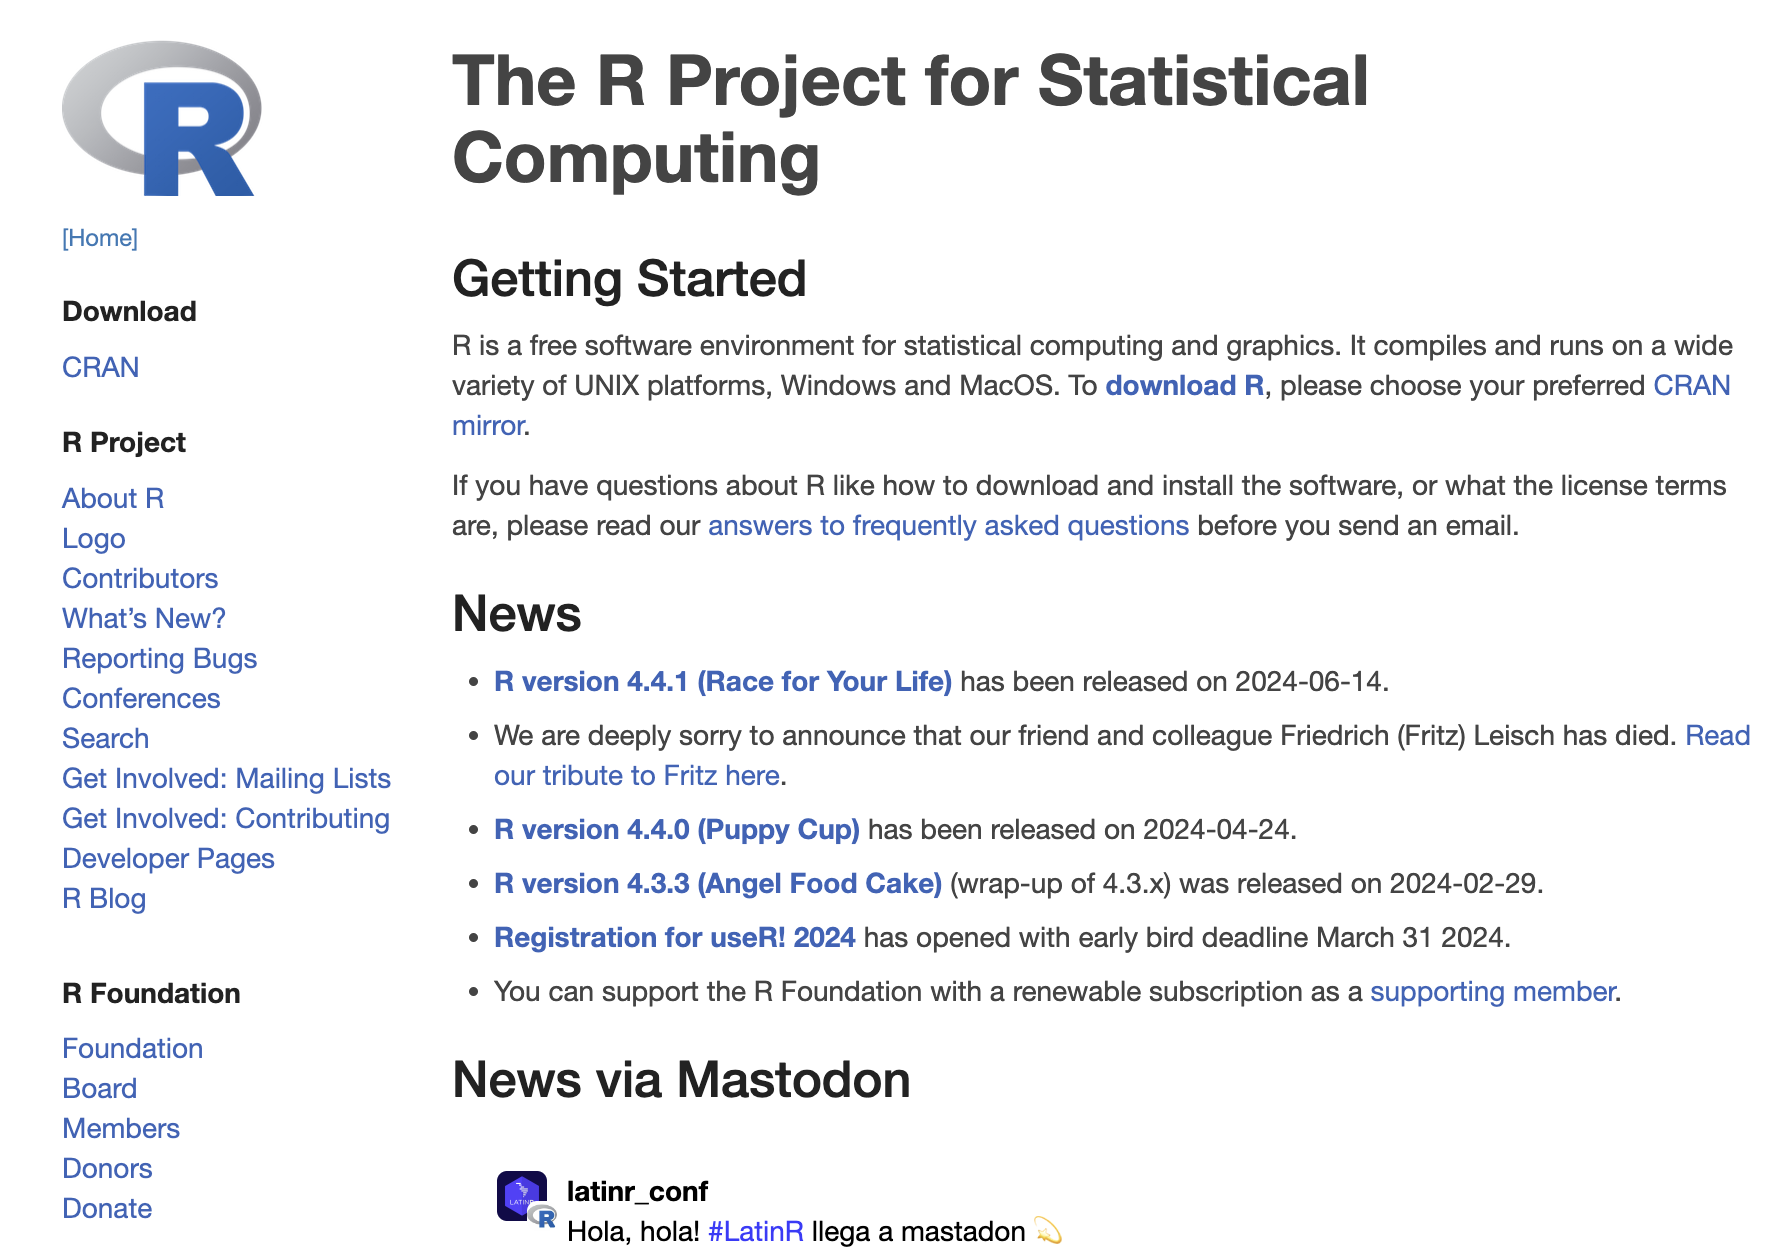
\includegraphics[width=0.8\textwidth,height=\textheight]{img/01_Rwebsite.png}
\end{center}

\end{minipage}%

\caption{\label{fig-Rwebsite}Website ของ R project}

\end{figure}%

เมื่อติดตั้งโปรแกรมเสร็จสมบูรณ์ และดำเนินการเปิดโปรแกรม ผู้อ่านจะพบกับหน้าต่างที่เรียกว่า R
Console ในรูป 1.2 หน้าต่างดังกล่าวมีหน้าที่ รับคำสั่ง/ข้อมูลเข้าสู่โปรแกรม
ส่งผ่านคำสั่งดังกล่าวไปยังหน่วยประมวลผลของเครื่อง รายงานผลลัพธ์/สถานะการทำงานต่าง ๆ
ให้กับผู้ใช้ การป้อนคำสั่งในหน้าต่าง Console สามารถทำได้โดยพิมพ์คำสั่งไว้
ที่บริเวณด้านหลังเครื่องหมาย \textgreater{} (เรียกว่าเครื่องหมาย prompt)
โดยเมื่อพิมพ์คำสั่งเสร็จแล้วให้ผู้ใช้ กดปุ่ม Enter โปรแกรมจะทำการประมวลผล
และแสดงผลลัพธ์ในบรรทัดถัดไป อย่างไรก็ตามการ เขียนคำสั่งใน R console
มีข้อจำกัดประการหนึ่งคือผู้ใช้สามารถเขียนคำสั่งและประมวลได้ทีละ บรรทัด
ผู้ใช้สามารถประมวลผลหลายคำสั่งภายในบรรทัดเดียวกันได้ โดยการใช้เครื่องหมาย semicolon
(;) คั่นระหว่างคำสั่ง เช่น 1+1; 2\^{}2+3; 2*3+4 และเมื่อกด Enter จะได้ผลลัพธ์ของ
คำสั่งทั้งหมดในคราวเดียว

\begin{figure}

\begin{minipage}{\linewidth}

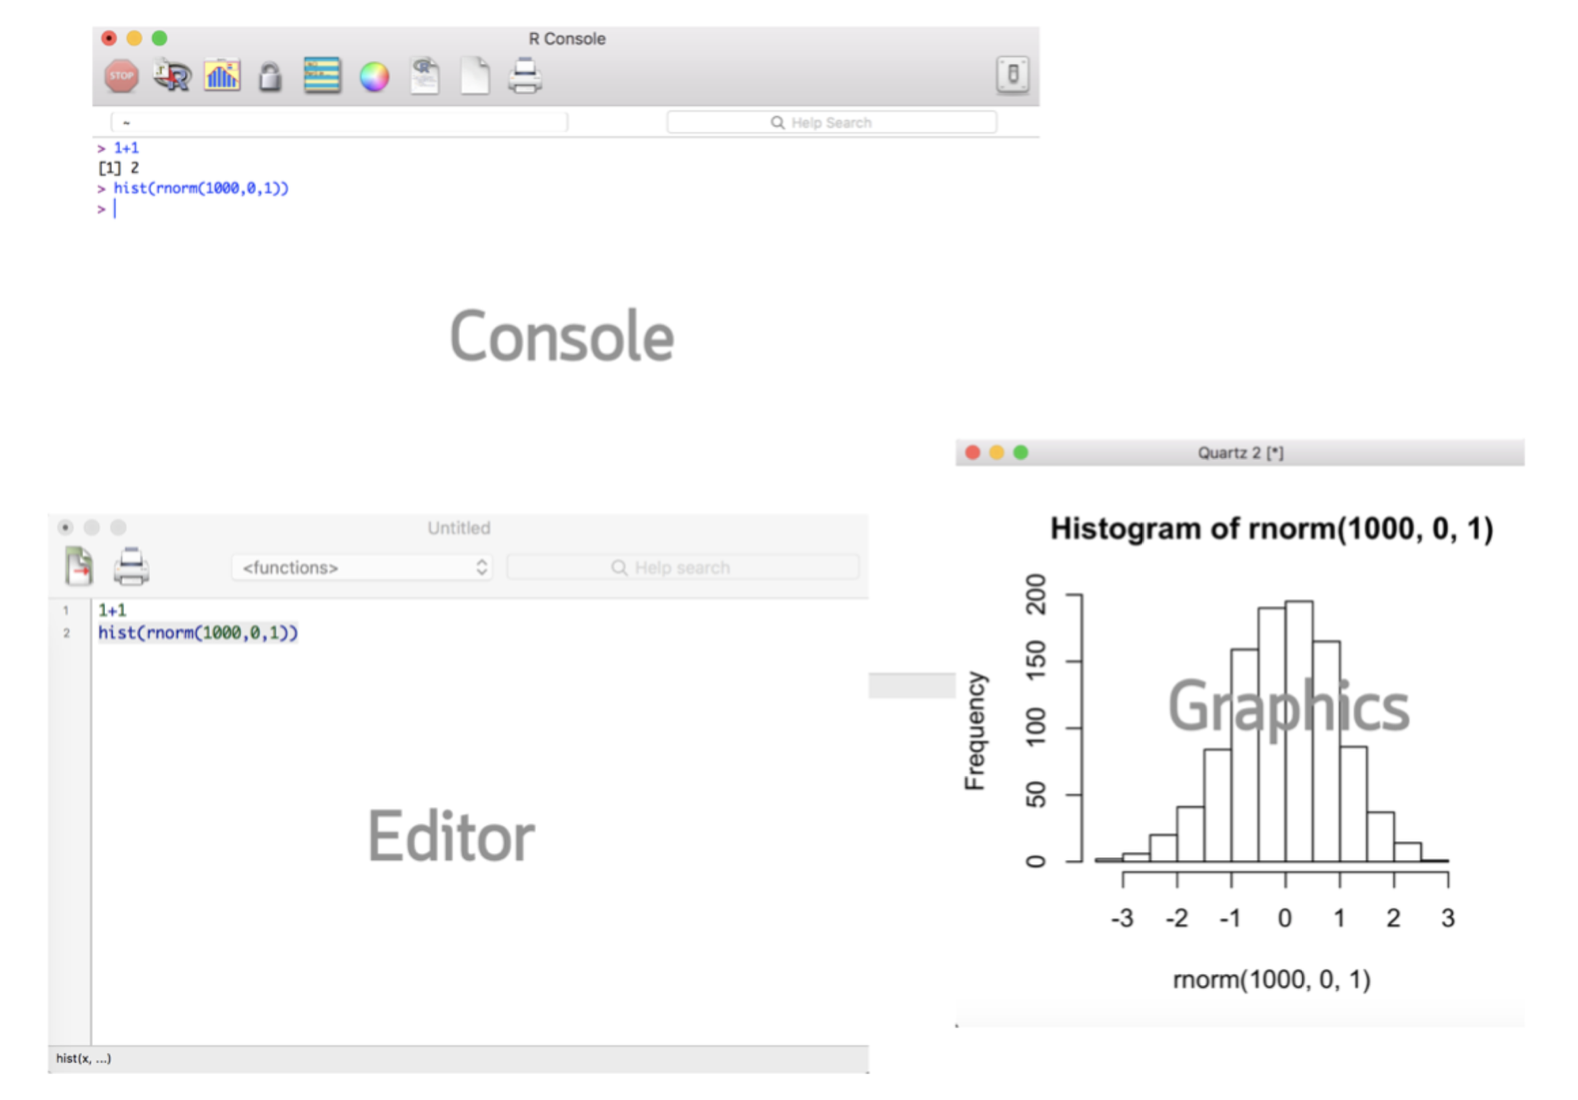
\includegraphics[width=0.8\textwidth,height=\textheight]{img/01_Renvironment.png}

\end{minipage}%

\caption{\label{fig-REnvironment}สภาพแวดล้อมของ R}

\end{figure}%

จากข้อจำกัดในการทำงานบนหน้าต่าง Console ข้างต้น จึงมีการพัฒนาหน้าต่าง Editor
ขึ้นเพื่อใช้สำหรับใช้เขียนชุดคำสั่งที่มีความซับซ้อนเข้าสู่โปรแกรม หน้าต่าง Editor ยอมให้ผู้ใช้
สามารถป้อนคำสั่งหรือข้อมูลได้หลายบรรทัด โดยยังไม่จำเป็นต้องสั่งประมวลผลในทันที สามารถ
เลือกประมวลผลคำสั่งทีละบรรทัด บางบรรทัด หรือทุกบรรทัดได้อย่างอิสระตามความต้องการ
นอกจากนี้คำสั่งที่เขียนในหน้าต่าง Editor ยังสามารถเก็บบันทึกไว้ในไฟล์นามสกุล .R (โดยทั่วไป
เรียกว่า script file) ซึ่งช่วยให้ผู้ใช้สามารถจัดระเบียบในการทำงานได้ สามารถสืบค้นย้อน
ประวัติการทำงานจากคำสั่งที่เขียนไว้ก่อนหน้าได้ นอกจากนี้ยังสามารถนำกลับมาใช้ซ้ำ แก้ไข หรือ
ดัดแปลงให้เหมาะสำหรับการทำงานอื่น ๆ ต่อไปได้อีกด้วย

หน้าต่าง Editor นี้ไม่ได้ปรากฏให้ผู้ใช้ใช้งานได้ทันทีเมื่อเปิดโปรแกรม ผู้ใช้จำเป็นต้อง
เรียกเปิดหน้าต่างดังกล่าวขึ้นมาใช้งานโดยคลิกเลือกที่เมนู File บนแถบเมนูด้านบน จากนั้นเลือก
New Script (สำหรับระบบปฏิบัติการ Windows) หรือเลือก New Document (สำหรับระบบ
ปฏิบัติการ Mac OS) โดยหากต้องการให้ R ประมวลคำสั่งในบรรทัดใด ให้ผู้ใช้คลิกเลือกคำสั่งหรือ
ทำ highlight คลุมบรรทัดของคำสั่งที่ต้องการประมวลผล จากนั้นกดปุ่ม Clt+R (สำหรับระบบ
ปฏิบัติการ Windows) หรือกดปุ่ม ⌘+Enter (สำหรับระบบปฏิบัติการ Mac OS)

หน้าต่างสุดท้ายเรียกว่าหน้าต่าง Graphics (สำหรับระบบปฏิบัติการ Mac OS เรียก หน้าต่างนี้ว่า
Quartz) เป็นหน้าต่างสำหรับแสดงผลลัพธ์เชิงกราฟิกที่ประมวลผลได้จากโปรแกรม
ผู้ใช้จะพบกับหน้าต่างนี้เมื่อมีการเรียกใช้คำสั่งที่ให้ผลลัพธ์เชิงกราฟิก ดังตัวอย่างในรูป 1.2 ที่แสดง
การสร้าง histogram เพื่อสำรวจการแจกแจงของข้อมูลจำลองจากเลขสุ่มที่มีการแจกแจงแบบปกติ
มาตรฐานจำนวน 1000 ค่าโดยใช้ฟังก์ชัน \texttt{hist()}

\section{RStudio IDE}\label{rstudio-ide}

ปัจจุบันการทำงานในโครงการหรืองานวิจัยที่มีการใช้สถิติและวิทยาการข้อมูล
ผู้วิเคราะห์จะต้องเกี่ยวข้องกับการใช้เครื่องมือและเทคนิคจำนวนมากและหลากหลาย
ทำให้การทำงานภายใต้สภาพแวดล้องของ R
โดยตรงอาจทำได้ยากโดยเฉพาะในกลุ่มผู้ใช้ที่ไม่ได้เชี่ยวชาญการเขียนโปรแกรม
นอกจากนี้ยังอาจมีความยากในการบริหารจัดการไฟล์ข้อมูลและไฟล์ที่เกี่ยวข้องกับการดำเนินงาน

จากความจำเป็นดังกล่าวจึงมีการพัฒนาโปรแกรมประเภท IDE (Integrated Development
Environment) ขึ้นเพื่อให้ผู้ใช้ R
มีเครื่องมือหรือตัวช่วยในการเขียนคำสั่งหรือพัฒนาโปรแกรมการวิเคราะห์ข้อมูลได้ง่ายและมีประสิทธิภาพมากขึ้น
โดย Rstudio มีคุณสมบัติที่เป็นจุดเด่นดังนี้

\begin{enumerate}
\def\labelenumi{\arabic{enumi}.}
\item
  RStudio มีสภาพแวดล้อมที่เป็นมิตรกับผู้ใช้มากขึ้น
  โดยมีการออกแบบส่วนตอบสนองกับผู้ใช้ที่มีการวางเครื่องมืออำนวยความสะดวกในการสั่งการทำงานของโปรแกรม
  R ทำให้การดำเนินการหลายส่วนสามารถทำได้โดยไม่จำเป็นต้องเขียนชุดคำสั่ง
  ซึ่งช่วยลดระยะเวลาการทำงานและทำให้ใช้งานภาษา R ได้ง่ายมากขึ้น เช่น
  การติดตั้งและเรียกใช้ library ต่าง ๆ การค้นหาไฟล์ข้อมูล การนำเข้าไฟล์ข้อมูล และ
  เรียกดูข้อมูลของตัวแปร
\item
  มีตัวแก้ไขคำสั่ง (Script Editor) ที่มีประสิทธิภาพสูงขึ้น โดยมีจุดเด่นที่เหนือกว่าการใช้ R
  Editor หลายประการ เช่น
  การเน้นสีของไวยกรณ์ภาษาทำให้การตรวจสอบแก้ไขคำสั่งสามารถทำได้ง่ายมากขึ้น
  การแนะนำคำสั่งที่เป็นไปได้ การแแจ้งเตือนและตรวจสอบข้อผิดพลาด นอกจากนี้ Editor ของ
  Rstudio ยังสามารถทำงานร่วมกับ Github Copilot ที่เป็น AI
  ที่ถูกฝึกสอนมาให้มีความสามารถในการช่วยสร้างคำสั่งซึ่งทำให้การทำงานด้านวิทยาการข้อมูลมีความสะดวกสบาย
  และมีประสิทธิภาพขึ้นอย่างมาก
\item
  การจัดการ workspace และไฟล์ที่เกี่ยวข้อง RStudio จะจัดการ workspace
  และไฟล์ทั้งหมดที่เกี่ยวข้องกับโปรเจคในโฟลเดอร์เดียว ทำให้การจัดการไฟล์มีความเป็นระบบ
  และลดความสับสนเมื่อทำงานกับหลายโปรเจค
\item
  การจัดการเวอร์ชัน (version control) RStudio รองรับการใช้งานร่วมกับ Git
  ภายในโปรเจค ทำให้สามารถควบคุมเวอร์ชันของโค้ดได้อย่างมีประสิทธิภาพ เช่น การ
  commit, push, pull, และดูประวัติการเปลี่ยนแปลงของโค้ดได้จากภายใน RStudio
  โดยตรง
\item
  RStudio รองรับการใช้งาน R Markdown และ Quarto
  ซึ่งเป็นเครื่องมือที่ช่วยให้ผู้ใช้สามารถสร้างเอกสารที่รวมโค้ด, ข้อความ,
  และผลลัพธ์ไว้ในไฟล์เดียวกัน สามารถสร้างรายงานแบบทำซ้ำได้ (reproducible report)
  ในรูปแบบต่าง ๆ เช่น เอกสารรายงาน/บทความ หนังสือ สไลด์นำเสนองาน และ เว็ปไซด์
\end{enumerate}

เมื่อเปิด RStudio ขึ้นมาผู้ใช้จะพบกับหน้าต่างหรือสภาพแวดล้อมดังรูป 1.3 ที่แบ่งออกเป็น 4 ส่วน
ได้แก่ \textbf{(1) Source} เป็นส่วนสำหรับใช้เขียนคำสั่ง (scripts) เขียน markdown
หรือเอกสาร quarto
ซึ่งทำให้ผู้ใช้สามารถจัดการกับโค้ดได้อย่างเป็นระบบสามารถสั่งรันโค้ดบางส่วนหรือทั้งไฟล์ได้อย่างสะดวก
ในทำนองเดียวกับ R Editor หากต้องการให้ R ประมวลคำสั่งในบรรทัดใด
ให้ผู้ใช้คลิกเลือกคำสั่งหรือ ทำ highlight คลุมบรรทัดของคำสั่งที่ต้องการประมวลผล
จากนั้นกดปุ่ม Clt+R (สำหรับระบบปฏิบัติการ Windows) หรือกดปุ่ม ⌘+Enter
(สำหรับระบบปฏิบัติการ Mac OS) \textbf{(2) Console}
เป็นส่วนที่แสดงผลลัพธ์จากการรันโค้ดหรือคำสั่งต่างๆ
โดยผู้ใช้สามารถพิมพ์คำสั่งโดยตรงเพื่อให้รันทันทีได้ที่นี่ \textbf{(3) Environment/History}
ในส่วนนี้จะแสดงข้อมูลของตัวแปรต่างๆ ที่ถูกสร้างขึ้นใน session ของการทำงาน
รวมถึงประวัติของคำสั่งที่ถูกใช้ไปก่อนหน้านี้ ช่วยให้ผู้ใช้สามารถย้อนดูหรือเรียกใช้คำสั่งเดิมได้ง่าย
และ \textbf{(4) Files/Plots/Packages/Help/Viewer} เป็นส่วนสำหรับการจัดการไฟล์
การดูกราฟหรือแผนภาพที่สร้างขึ้น การจัดการ package/library ที่ติดตั้ง
การค้นหาความช่วยเหลือใน R และการแสดงผลข้อมูลที่เกี่ยวข้อง เช่น ไฟล์ HTML
หรือไฟล์ภาพที่ถูกสร้างขึ้น

\begin{figure}

\begin{minipage}{0.50\linewidth}

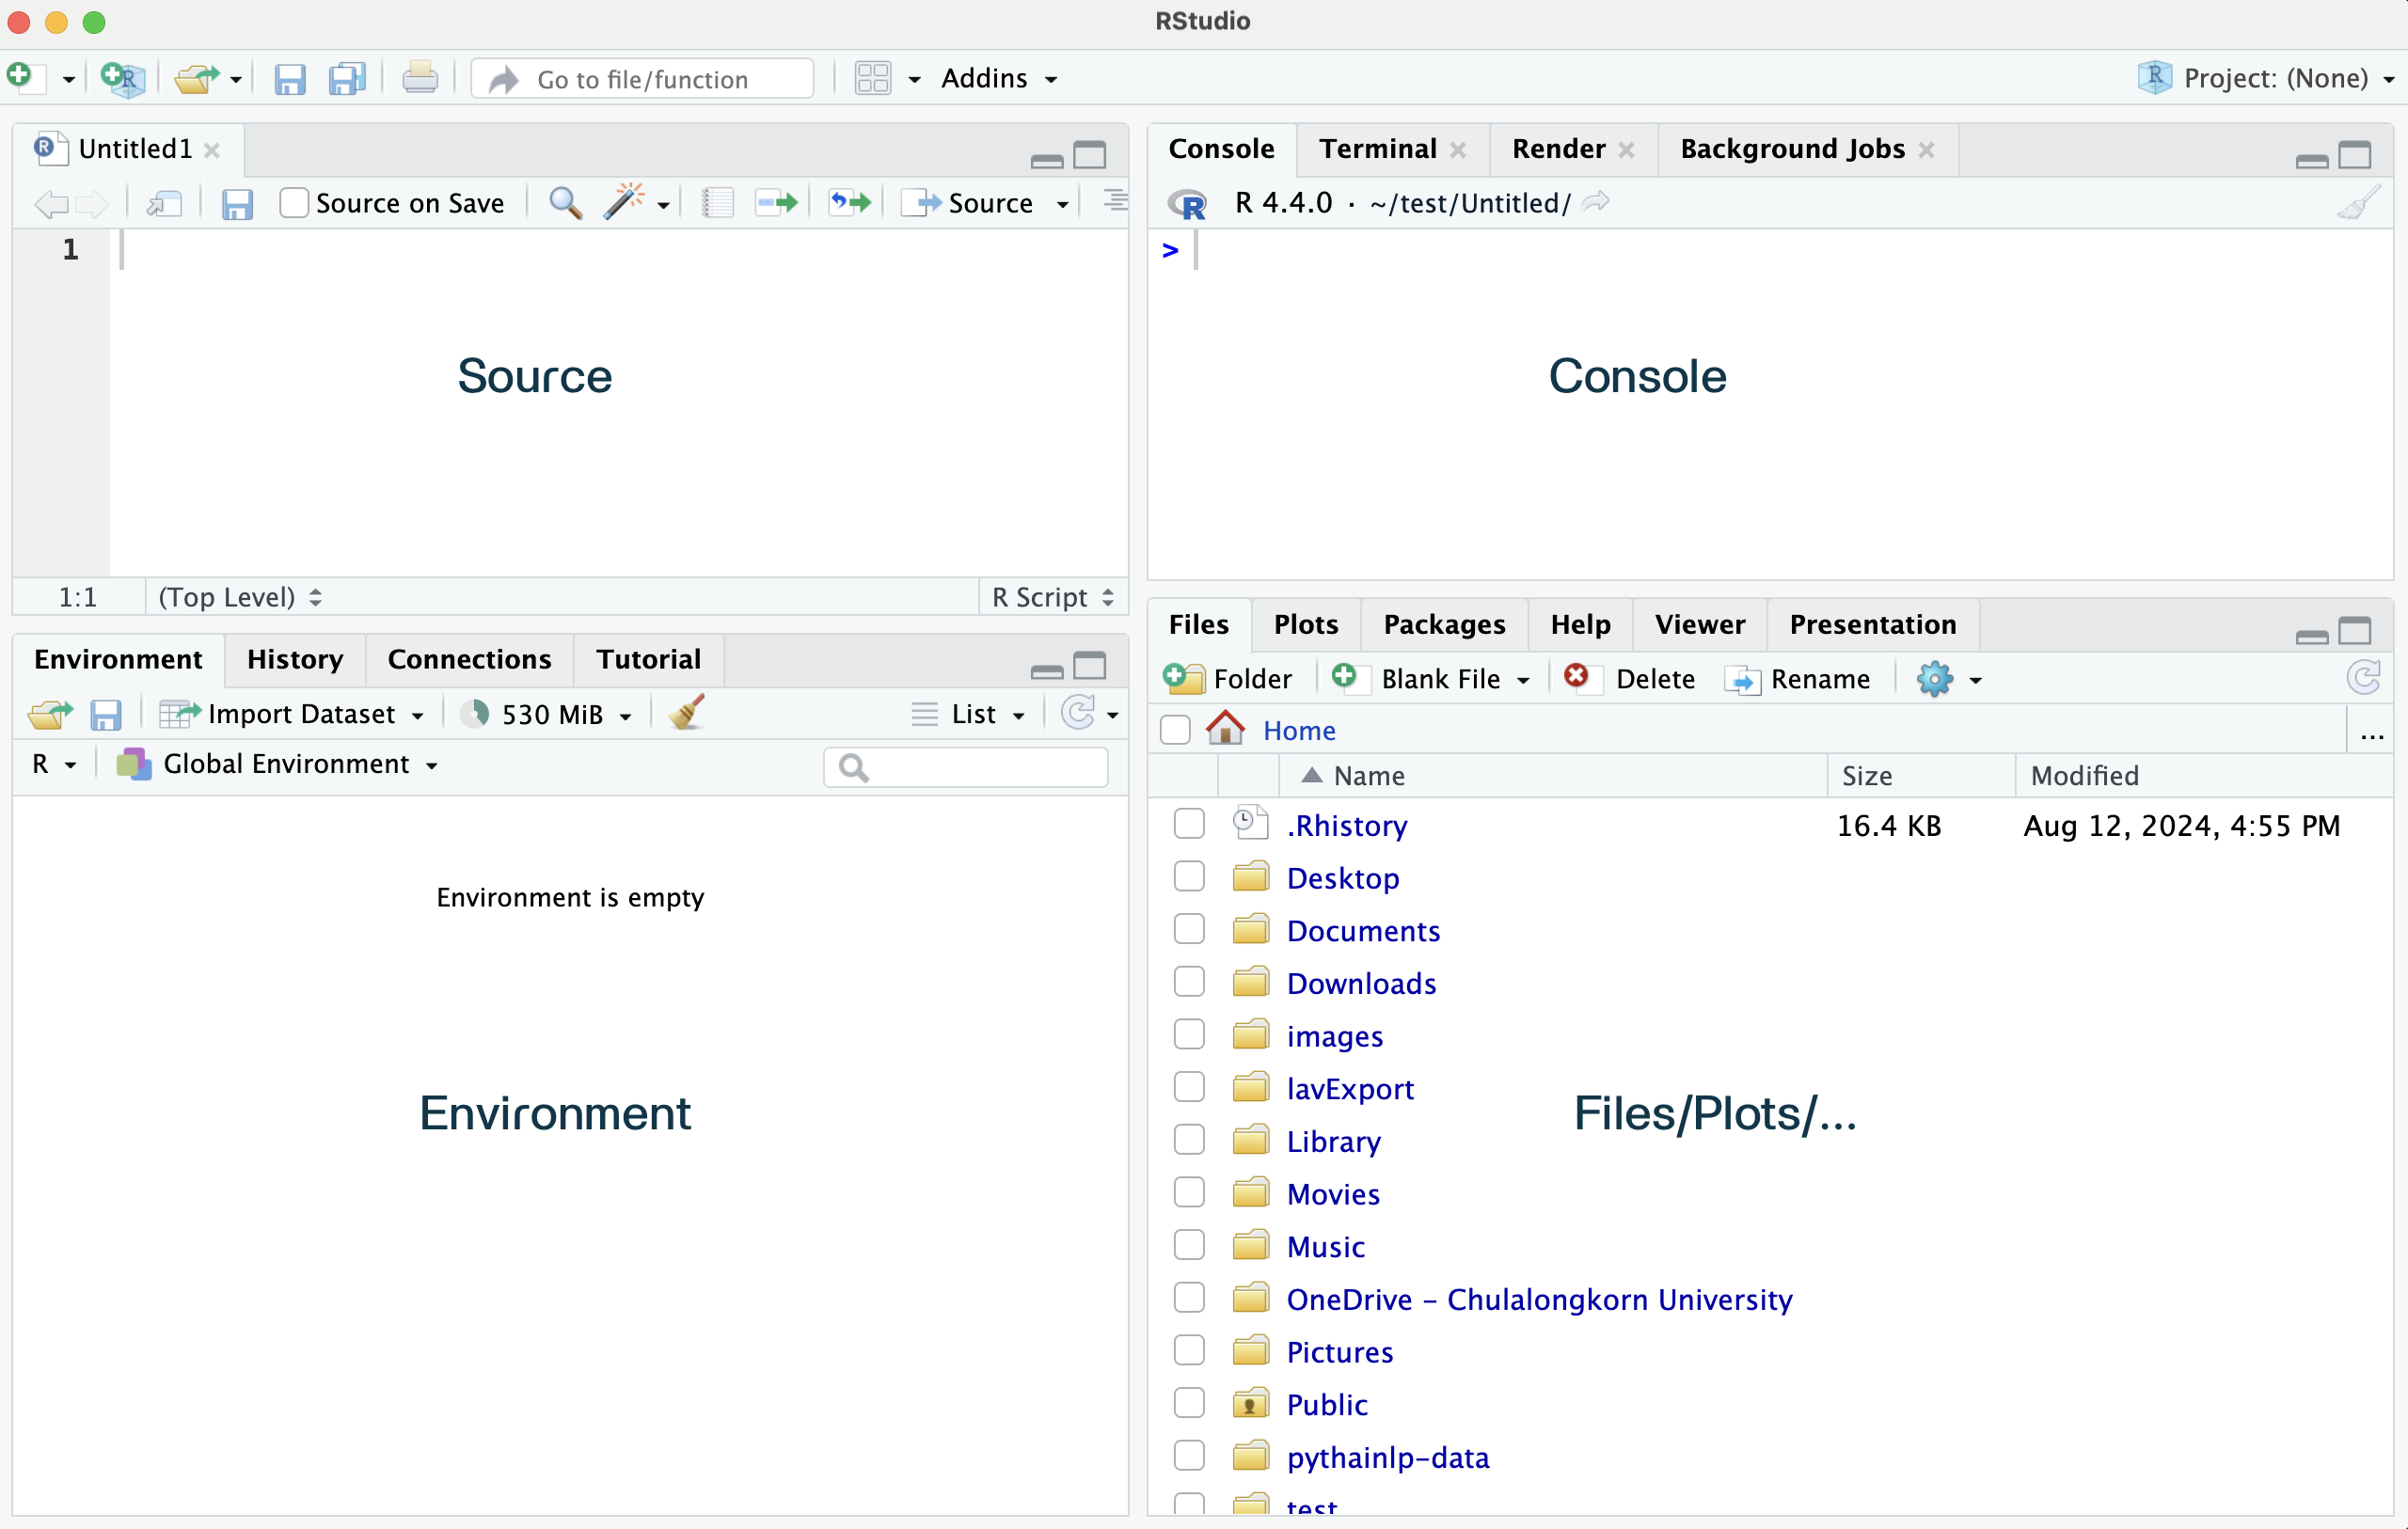
\includegraphics{img/01Rstudio.png}

\subcaption{\label{}RStudio}
\end{minipage}%
%
\begin{minipage}{0.50\linewidth}

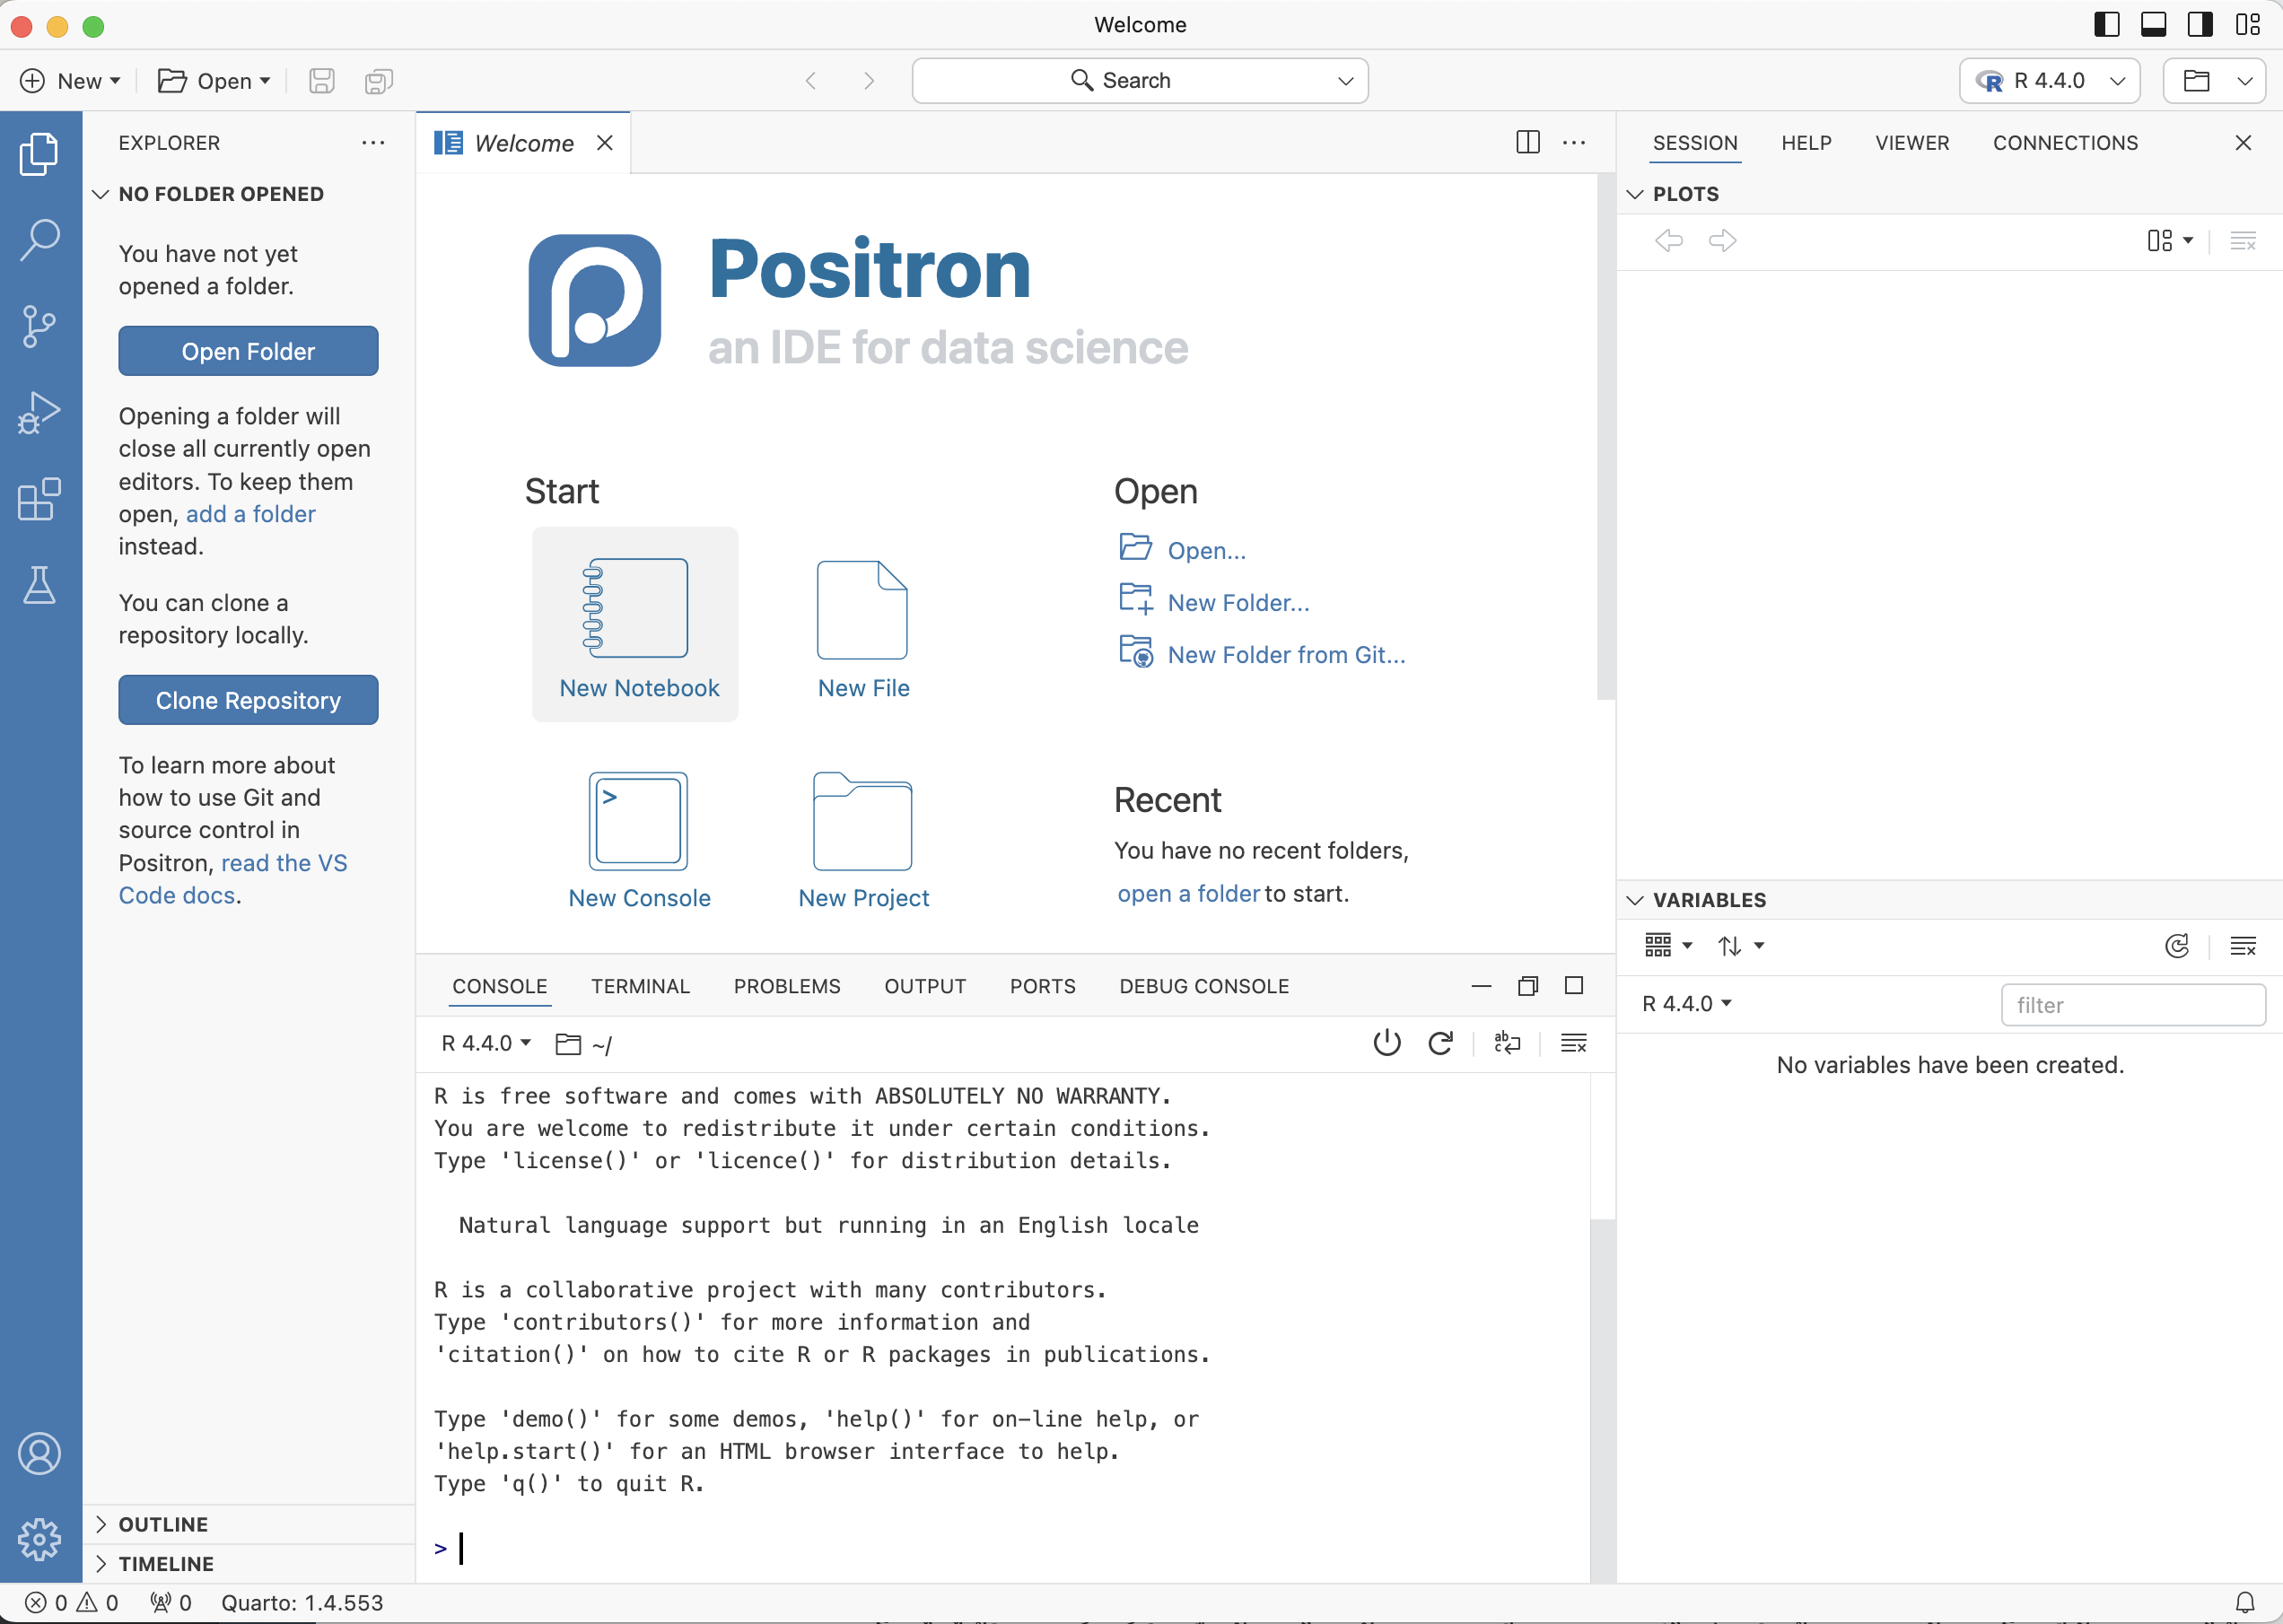
\includegraphics[width=0.9\textwidth,height=\textheight]{img/01Positron.png}

\subcaption{\label{}Positron}
\end{minipage}%

\caption{\label{fig-IDE}สภาพแวดล้อมของ IDE}

\end{figure}%

ผู้ใช้สามารถเข้าไปดาวน์โหลด RStudio ได้ที่
\url{https://posit.co/download/rstudio-desktop/} ทั้งนี้ก่อนการติดตั้ง RStudio
ผู้ใช้จำเป็นจะต้องมีโปรแกรม R ตัวพื้นฐานติดตั้งอยู่ในเครื่องก่อนแล้ว

\section{Positron IDE}\label{positron-ide}

Positron ได้การนิยามตัวเองว่าเป็น IDE
สำหรับวงการวิทยาการข้อมูลที่รองรับการเขียนโปรแกรมหลากหลายภาษา ออกแบบมาเพื่อผู้ใช้ VS
Code หรือ JupyterLab ที่ทำงานด้านวิทยาการข้อมูลด้วยภาษา Python หรือ R
แต่ยังรู้สึกไม่พอใจกับฟีเจอร์หรือความสามารถในการปรับแต่งที่มีอยู่เดิม Positron
เน้นการใช้งานหลักในภาษา Python และ R พร้อมความสามารถในการเพิ่มภาษาอื่น ๆ
ผ่านส่วนขยาย (รองรับส่วนขยายของ VS Code) โครงการ Positron
นี้พัฒนาในรูปแบบโอเพนซอร์สบน GitHub และยังคงพัฒนาโดยบริษัท Posit ควบคู่ไปกับ RStudio
โดยไม่ได้ทิ้งซอฟต์แวร์เดิมเพื่อพัฒนาใหม่ทั้งหมด ขณะนี้ Positron อยู่ในช่วงเริ่มต้นของการพัฒนา
โดยมีลักษณะการใช้งานคล้ายกับ VS Code ที่รองรับ Python และ R
โดยไม่ต้องติดตั้งส่วนขยายเพิ่มเติม Posit
มีแผนที่จะเพิ่มฟีเจอร์สำหรับงานวิทยาการข้อมูลเพิ่มเติมในอนาคต

สภาพแวดล้อมใน Positron มีโครงสร้างคล้ายกับ Rstudio
และมีหน้าต่างย่อยสำหรับทำงานที่คล้ายคลึงกันรูป 1.4 แสดงสภาพแวดล้อมของ Positron

ผู้ใช้สามารถดาวน์โหลด Positrion ได้ที่
\url{https://github.com/posit-dev/positron/releases}
และสามารถติดต่อข่าวสารและรายละเอียดเกี่ยวกับ Positron ได้ที่
\url{https://github.com/posit-dev/positron?tab=readme-ov-file}

\section{ควรใช้ RStudio หรือ
Positron}\label{uxe04uxe27uxe23uxe43uxe0a-rstudio-uxe2buxe23uxe2d-positron}

\ldots{}

\bookmarksetup{startatroot}

\chapter{พื้นฐาน R}\label{uxe1euxe19uxe10uxe32uxe19-r}

เมื่อผู้อ่านดาวน์โหลดและติดตั้งโปรแกรม R รวมทั้ง RStudio หรือ Positron แล้ว
บทเรียนนี้จะกล่าวถึงการใช้ภาษาเบื้องต้น ได้แก่ การคำนวณทางคณิตศาสตร์พื้นฐาน ฟังก์ชัน
มโนทัศน์เกี่ยวกับตัวแปรในภาษา R ประเภทของตัวแปรและการสร้างตัวแปร
และการอ้างอิงค่าหรือสมาชิกภายในตัวแปรที่สร้างขึ้น
ในการเรียนรู้และประมวลผลคำสั่งตามเนื้อหาในบทเรียนนี้ ผู้อ่านสามารถพิมพ์คำสั่งบนเอกสาร
Script โดยหากใช้ RStudio ผู้อ่านสามารถเปิดเอกสาร Script ได้โดยคลิกที่แถบเมนูด้านบน
File --\textgreater{} New File --\textgreater{} R Script สำหรับใน
Positron ให้สร้างไฟล์เอกสาร .R โดยบนแถบเมนูให้คลิกที่ File --\textgreater{} New
File --\textgreater{} R File R ดังรูป 2.1

\begin{figure}

\begin{minipage}{0.50\linewidth}

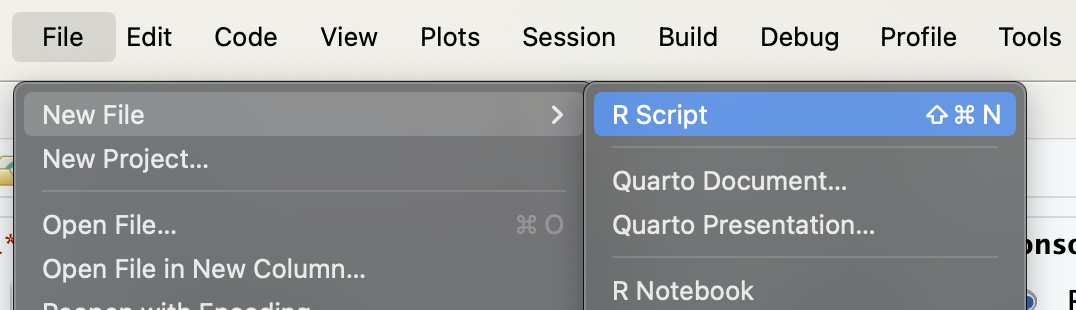
\includegraphics[width=1\textwidth,height=\textheight]{img/02Rscript.png}

\subcaption{\label{}Rstudio}
\end{minipage}%
%
\begin{minipage}{0.50\linewidth}

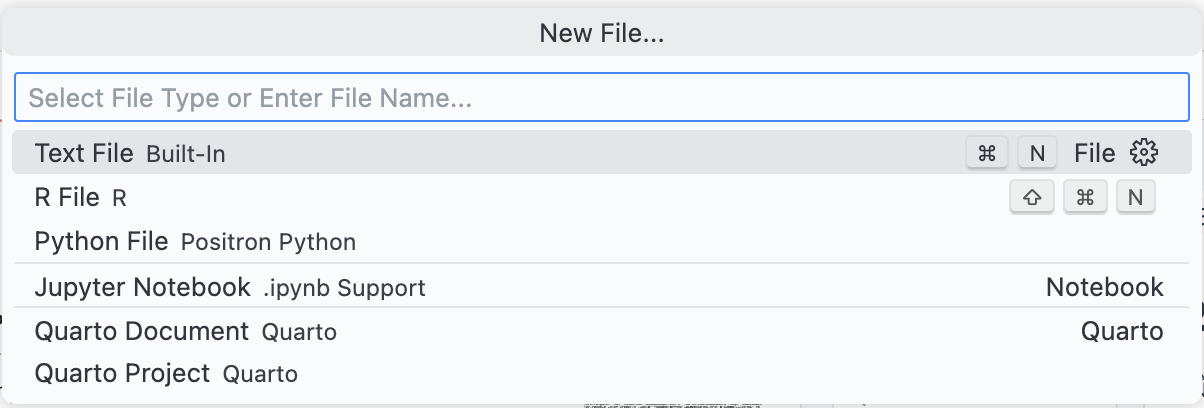
\includegraphics[width=0.88\textwidth,height=\textheight]{img/02.R_positron.png}

\subcaption{\label{}Positron}
\end{minipage}%

\caption{\label{fig-IDE}การเปิดหน้าต่าง Editor หรือ Script ใน IDE}

\end{figure}%

รายละเอียดมีดังนี้

\section{การคำนวณทางคณิตศาสตร์พื้นฐาน}\label{uxe01uxe32uxe23uxe04uxe33uxe19uxe27uxe13uxe17uxe32uxe07uxe04uxe13uxe15uxe28uxe32uxe2auxe15uxe23uxe1euxe19uxe10uxe32uxe19}

ภาษา R มีฟังก์ชันพื้นฐานสำหรับการคำนวณทางคณิตศาสตร์จำนวนมาก เช่น การ
ดำเนินการพีชคณิตพื้นฐานได้แก่ การบวก (+) ลบ (-) คูณ (*) หาร (/) ยกกำลัง (\^{})
และ รากที่ สอง (\texttt{sqrt()}) รวมทั้งการคำนวณผลลัพธ์จากฟังก์ชันอดิศัย (implicit
function) ต่าง ๆ เช่น ฟังก์ชันตรีโกณมิติ \texttt{sin()}, \texttt{cos()},
\texttt{tan()} ฟังก์ชันลอการิทึมธรรมชาติ \texttt{log()} ฟังก์ชันเอกซ์ โพเนนเซียล
\texttt{exp()} และ วงเล็บ \texttt{(\ )} เป็นต้น
ชุดคำสั่งด้านล่างแสดงตัวอย่างการดำเนินการทาง คณิตศาสตร์ใน R
ผู้อ่านลองพิมพ์คำสั่งดังกล่างลงในเครื่องคอมพิวเตอร์ของตนเอง จากนั้นสังเกต ผลลัพธ์ที่ได้

\begin{Shaded}
\begin{Highlighting}[]
\DecValTok{1}\SpecialCharTok{+}\DecValTok{1}\NormalTok{; }\DecValTok{3{-}2}\NormalTok{; }\DecValTok{4}\SpecialCharTok{*}\DecValTok{5}\NormalTok{; }\DecValTok{10}\SpecialCharTok{/}\DecValTok{2}
\DecValTok{3}\SpecialCharTok{\^{}}\DecValTok{3}\NormalTok{; }\FunctionTok{sqrt}\NormalTok{(}\DecValTok{625}\NormalTok{); }\DecValTok{81}\SpecialCharTok{\^{}}\NormalTok{(}\DecValTok{1}\SpecialCharTok{/}\DecValTok{3}\NormalTok{)}
\DecValTok{5}\SpecialCharTok{\%\%}\DecValTok{3}\NormalTok{; (}\DecValTok{3}\SpecialCharTok{\^{}}\DecValTok{3}\SpecialCharTok{+}\DecValTok{5{-}1}\NormalTok{)}
\FunctionTok{log}\NormalTok{(}\DecValTok{10}\NormalTok{); }\FunctionTok{exp}\NormalTok{(}\DecValTok{5}\NormalTok{)}
\end{Highlighting}
\end{Shaded}

\section{ฟังก์ชัน (functions)}\label{uxe1fuxe07uxe01uxe0auxe19-functions}

ในหัวข้อที่ผ่านมาจะเห็นว่ามีการใช้งานฟังก์ชันในโปรแกรม R ไปบางตัวทั้งฟังก์ชันทาง คณิตศาสตร์
เช่น \texttt{sqrt()}, \texttt{exp()} และ \texttt{log()} และฟังก์ชันกราฟิกคือ
\texttt{hist()} เป็นต้น ผู้
อ่านจะสังเกตว่าการใช้ฟังก์ชันดังกล่าวในการทำงานช่วยให้ผู้ใช้ลดขั้นตอนในการทำงานที่ไม่
จำเป็นไปได้ นอกจากนี้ยังช่วยให้ syntax ของผู้เขียนโปรแกรมสั้นลง ทำงานได้ไวขึ้นและมี
ประสิทธิภาพสูงขึ้น เช่นหากต้องการหาค่าสัมบูรณ์ของ -10 ในกรณีที่ไม่ได้ฟังก์ชันเข้ามาช่วยใน
การประมวลผล ผู้วิเคราะห์จำเป็นต้องเขียนอัลกอริทึมเพื่อหาค่าสัมบูรณ์เองโดยอาจใช้คำสั่ง IF,
ELSE เพื่อควบคุมเงื่อนไขการทำงานของ R ดังตัวอย่างคำสั่งด้านล่าง ซึ่งจะได้ผลลัพธ์เท่ากับ 10

\begin{Shaded}
\begin{Highlighting}[]
\NormalTok{x}\OtherTok{\textless{}{-}}\NormalTok{(}\SpecialCharTok{{-}}\DecValTok{10}\NormalTok{)}
\DocumentationTok{\#\# เขียนกระบวนการเพื่อหา absolute ของ x}
\ControlFlowTok{if}\NormalTok{(x}\SpecialCharTok{\textless{}}\DecValTok{0}\NormalTok{)\{}\SpecialCharTok{{-}}\NormalTok{(x)\} }\ControlFlowTok{else}\NormalTok{ \{x\}}
\end{Highlighting}
\end{Shaded}

\begin{verbatim}
[1] 10
\end{verbatim}

อย่างไรก็ตามเมื่อเปรียบเทียบกับการใช้ฟังก์ชันเข้ามาช่วยในการทำงาน โดยในกรณีนี้นำ
เอาฟังก์ชัน abs() เข้ามาช่วยคำนวณค่าสัมบูรณ์ ผู้อ่านจะเห็นว่าการเขียนคำสั่งลดลงเหลือเพียง
บรรทัดเดียวเท่านั้น ดังนี้

\begin{Shaded}
\begin{Highlighting}[]
\FunctionTok{abs}\NormalTok{(}\SpecialCharTok{{-}}\DecValTok{10}\NormalTok{)}
\end{Highlighting}
\end{Shaded}

\begin{verbatim}
[1] 10
\end{verbatim}

จากตัวอย่างในข้างต้นผู้อ่านจะสังเกตเห็นว่าการใช้ฟังก์ชันในการดำเนินงานช่วยลดขั้น
ตอนและประหยัดเวลาในการทำงานได้อย่างมาก ในสภาพแวดล้อมการทำงานบนโปรแกรม R
\textbf{ฟังก์ชัน (function)} คือชุดคำสั่งสำเร็จรูปที่ถูกพัฒนาขึ้นสำหรับการทำงานเฉพาะด้าน
การใช้ ฟังก์ชันในการดำเนินงานจะช่วยให้ผู้ใช้ประหยัดเวลา ลดความผิดพลาดในการทำงาน
และทำให้ กระบวนการทำงานมีประสิทธิภาพมากยิ่งขึ้น ฟังก์ชันในโปรแกรม R
ไม่ได้จำกัดการใช้งานแต่ด้าน การคำนวณทางคณิตศาสตร์เท่านั้น
แต่ยังมีฟังก์ชันที่สามารถใช้ดำเนินงานลักษณะอื่นได้อีกหลาย ประเภท เช่น การคัดเลือกตัวแปร
การคัดกรองข้อมูล การสร้างแผนภาพหรือกราฟทางสถิติ และ
การประมวลผลเพื่อหาคำตอบในทางสถิติ เป็นต้น

ฟังก์ชันแต่ละตัวมีส่วนประกอบจำนวน 3 ส่วนหลัก ได้แก่ (1) ส่วนข้อมูลนำเข้า (input)
ส่วนนี้เป็นส่วนที่ผู้ใช้โปรแกรมต้องกำหนดหรือกรอกเข้าไปในฟังก์ชันเพื่อควบคุมการทำงานให้เป็น
ไปตามที่ต้องการ (2) ส่วนประมวลผล (process) ส่วนนี้เป็นส่วนการทำงานเบื้องหลัง ปกติแล้วผู้
ใช้มักจะไม่เห็นการทำงานในส่วนนี้ของฟังก์ชัน การประมวลผลนี้จะดำเนินการโดยขึ้นกับชุดคำสั่งที่
ผู้พัฒนาได้กำหนดไว้ และข้อมูลนำเข้าที่ผู้ใช้ระบุ และ (3) ส่วนผลลัพธ์ (output) เป็นผลลัพธ์หรือ
คำตอบที่ได้จากฟังก์ชัน ซึ่งอาจรายงานให้ผู้ใช้ทราบในหน้าต่าง Console ในทันที่ที่ประมวลผล
เสร็จสิ้น หรืออาจเก็บผลลัพธ์ดังกล่าวเอาไว้ในตัวแปร ซึ่งผู้ใช้จะต้องเรียกดูด้วยตนเองอีกครั้งหนึ่ง
โดยปกติการเรียกใช้ฟังก์ชันใน R มีรูปแบบคำสั่งดังนี้

\begin{Shaded}
\begin{Highlighting}[]
\FunctionTok{function\_name}\NormalTok{(arg1, arg2, ...)}
\end{Highlighting}
\end{Shaded}

โดยที่ \texttt{function\_name} คือชื่อของฟังก์ชัน และ \texttt{arg1} กับ
\texttt{arg2,\ ...} เป็นส่วนข้อมูลนำเข้าของ ฟังก์ชันเรียกว่า อาร์กิวเมนท์ (argument)
ใช้สำหรับป้อนข้อมูลที่จำเป็นและควบคุมการทำงานของ
ฟังก์ชันเพื่อให้ผลลัพธ์เป็นไปตามที่ผู้ใช้ต้องการ ทั้งนี้ฟังก์ชันสามารถมีอาร์กิวเมนท์ได้มากกว่าหนึ่ง
ตัวขึ้นอยู่กับลักษณะงานของแต่ละฟังก์ชัน ยกตัวอย่างเช่น ฟังก์ชัน
\texttt{log(x,\ base=exp(1))} ที่ มีอาร์กิวเมนท์ 2 ตัวได้แก่ \texttt{x} และ
\texttt{base} เมื่อกำหนดค่าทั้งสองฟังก์ชันจะหาค่า logarithm ของ ค่า \texttt{x}
เมื่อกำหนดฐานของ logarithm ให้มีค่าเท่ากับ \texttt{base} โดยในคำสั่งข้างต้นกำหนดให้
\texttt{base\ =\ exp(1)} ซึ่งมีค่าเท่ากับ \(e \approx 2.71828...\) เรียกว่า
natural logarithm ตัวอย่างด้านล่าง แสดงการหา ค่า natural logarithm ของ 10
ด้วยการใช้ฟังก์ชัน \texttt{log()} ข้างต้น

\begin{Shaded}
\begin{Highlighting}[]
\FunctionTok{log}\NormalTok{(}\AttributeTok{x =} \DecValTok{10}\NormalTok{, }\AttributeTok{base =} \FunctionTok{exp}\NormalTok{(}\DecValTok{1}\NormalTok{))}
\end{Highlighting}
\end{Shaded}

\begin{verbatim}
[1] 2.302585
\end{verbatim}

\begin{Shaded}
\begin{Highlighting}[]
\FunctionTok{log}\NormalTok{(}\DecValTok{10}\NormalTok{)}
\end{Highlighting}
\end{Shaded}

\begin{verbatim}
[1] 2.302585
\end{verbatim}

จากตัวอย่างข้างต้นผู้อ่านจะสังเกตเห็นว่าการเรียกใช้ฟังก์ชันใน R สามารถลดทอนการ
เขียนอาร์กิวเมนท์บางตัวได้ ในกรณีที่อาร์กิวเมนท์นั้นถูกกำหนดค่าเริ่มต้น (default value)
เอาไว้ จากตัวอย่างที่ผ่านมาจะเห็นว่า อาร์กิวเมนท์ base ถูกกำหนดค่าเริ่มต้น (default)
ให้มีค่าเท่ากับ \texttt{exp(1)} ระหว่างการเขียนคำสั่ง
\texttt{log(x,\ base=exp(1))} กับ \texttt{log(x)} จึงได้คำตอบเดียวกัน
ดังนั้นอาร์กิวเมนท์ \texttt{base} จึงเป็นอาร์กิวเมนท์ที่สามารถละการเขียนได้

\section{การเรียกคู่มือของฟังก์ชัน}\label{uxe01uxe32uxe23uxe40uxe23uxe22uxe01uxe04uxe21uxe2duxe02uxe2duxe07uxe1fuxe07uxe01uxe0auxe19}

R เป็นโปรแกรมที่มีฟังก์ชันให้เลือกใช้งานจำนวนมากในทางปฏิบัติจึงยากที่จะจำวิธีการใช้
ฟังก์ชันทั้งหมด การทำงานบนโปรแกรม R โดยปกติจึงมักมีการเรียกดูคู่มือการใช้ฟังก์ชันที่ใช้เป็น
ประจำ โดยผู้ใช้ R สามารถเรียกดูคู่มือของฟังก์ชันที่ต้องการได้โดยพิมพ์คำสั่ง ? ตามด้วยชื่อฟังก์ชัน
หรือใช้ฟังก์ชัน \texttt{help()} เพื่อเรียกดูคู่มือดังกล่าว เช่น หากต้องการเรียกดู คู่มือการใช้
ฟังก์ชัน \texttt{log()} ข้างต้นสามารถพิมพ์คำสั่งได้ดังนี้

\begin{Shaded}
\begin{Highlighting}[]
\NormalTok{?}\FunctionTok{log}\NormalTok{()}
\FunctionTok{help}\NormalTok{(log)}
\end{Highlighting}
\end{Shaded}

ตัวอย่างด้านล่างแสดงคู่มือการใช้งานฟังก์ชัน \texttt{log()} ข้างต้น เ

\begin{figure}

\begin{minipage}{\linewidth}

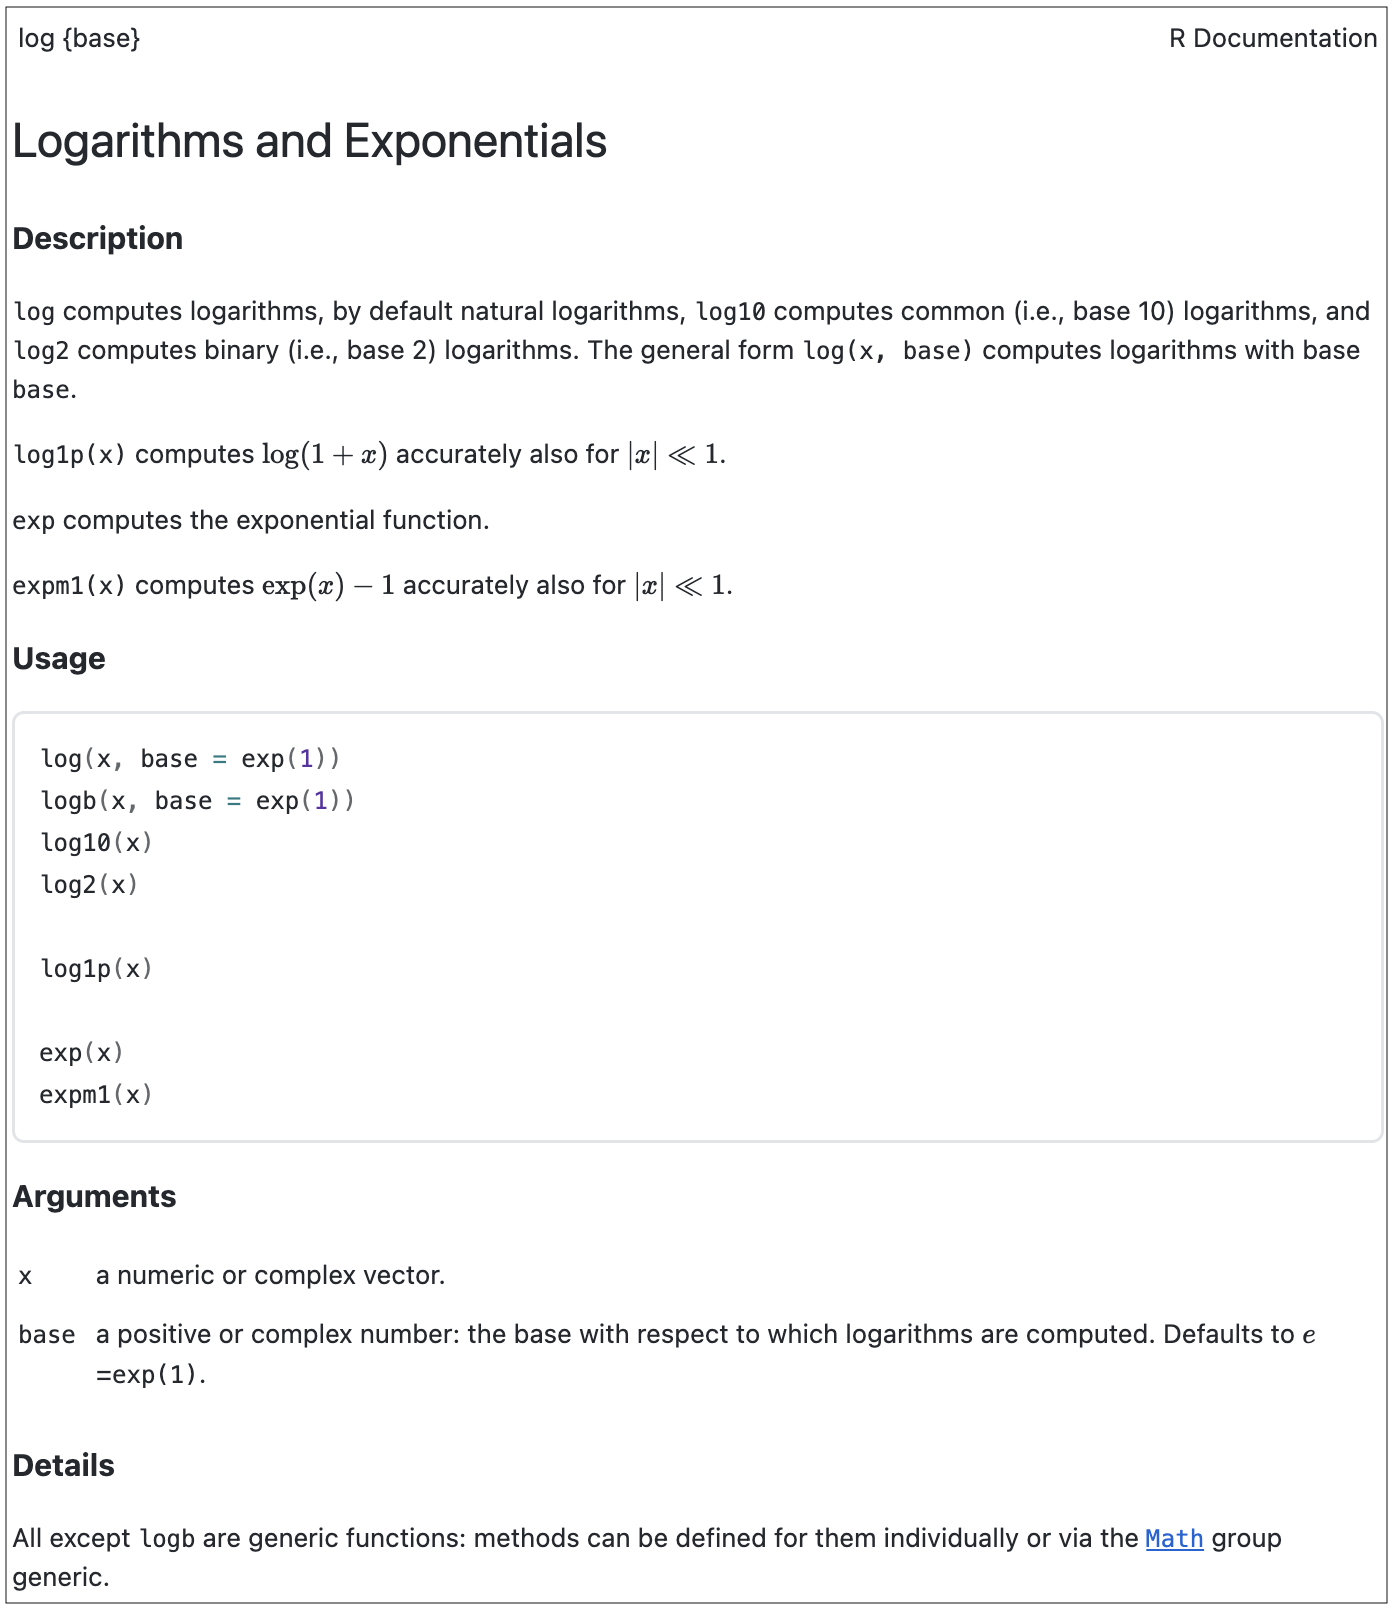
\includegraphics{img/02loghelp.png}

\end{minipage}%

\caption{\label{fig-Help}คู่มือการใช้งานฟังก์ชัน \texttt{log()}
ที่ได้จากการพิมพ์คำสั่ง \texttt{?log()}}

\end{figure}%

R มีฟังก์ชันจำนวนมากจากหลาย library สำหรับการทำงานในด้านวิทยาการข้อมูล
ในหนังสือเล่มนี้ผู้อ่านจะได้รู้จักและเรียนรู้การประยุกต์ใช้ฟังก์ชันต่าง ๆ
ที่จำเป็นในกระบวนการวิเคราะห์ข้อมูล ตั้งแต่การทำความสะอาดข้อมูล
การตรวจสอบข้อมูลที่ขาดหายไป การรวมและแยกข้อมูล การสร้างทัศนภาพข้อมูล
ไปจนถึงการคำนวณทางสถิติต่าง ๆ นอกจากการใช้ฟังก์ชันที่ผู้อื่นได้สร้างเอาไว้
ในบางกรณีผู้วิเคราะห์อาจจำเป็นจะต้องสร้างฟังก์ชันของตนเองเพื่อใช้ในการทำงานหรือเพื่อแก้ปัญหาต่าง
ๆ ซึ่งจะกล่าวถึงในประเด็นนี้อีกครั้งในส่วนท้ายของบทเรียนนี้
เนื้อหาส่วนถัดไปจะกล่าวถึงมโนทัศน์ของตัวแปรในภาษา R
ซึ่งพื้นฐานที่มีความสำคัญมากในการทำงานด้านสถิติและวิทยาการข้อมูล

\section{ตัวแปร (variables)}\label{uxe15uxe27uxe41uxe1buxe23-variables}

คำว่า ``ตัวแปร'' ภายใต้สภาพแวดล้อมของภาษา R มีความหมายที่แตกต่างไปจากตัวแปรใน
เชิงการวิจัยหรือการวิเคราะห์ข้อมูลทางสถิติ กล่าวคือ ตัวแปรเป็นวัตถุ (object)
ประเภทหนึ่งที่อยู่ภายใต้สภาพแวดล้อมของภาษา R
มีหน้าที่บันทึก/เก็บข้อมูลหรือผลลัพธ์ที่ได้จากการประมวลผลเอาไว้ในหน่วยความจำ ของคอมพิวเตอร์
ซึ่งทำให้ผู้ใช้สามารถเรียกดูค่าที่เก็บไว้ดังกล่าวในภายหลังหรือนำไปใช้ต่อใน
การดำเนินการขั้นตอนอื่น ๆ โดยไม่ต้องป้อนข้อมูลหรือประมวลผลใหม่ซ้ำ ๆ

ตัวแปรในภาษา R สามารถจำแนกได้หลากหลายประเภท ซึ่งทำให้การสร้างตัวแปร
และการดำเนินการสำหรับตัวแปรแต่ละประเภทมีรายละเอียดที่แตกต่างกันในบางส่วน หัวข้อนี้จะ
กล่าวถึงการสร้างตัวแปรพื้นฐานที่เรียกว่าตัวแปรสเกลาร์ (scalar) ที่ใช้เก็บข้อมูลได้หนึ่งค่าต่อ
ตัวแปร การสร้างตัวแปรแบบสเกลาร์ใน R สามารถทำได้โดยใช้คำสั่ง
\texttt{\textless{}-} (อ่านว่า assign) เช่น \texttt{x\textless{}-10}
หมายถึงกำหนดให้ R เก็บค่าคือ 10 ที่อยู่ทางส่วนปลายของลูกศรไว้ในตัวแปรชื่อ \texttt{x}
ที่อยู่ ทางส่วนหัวของลูกศร และเมื่อสร้างตัวแปร \texttt{x} ในข้างต้นแล้ว
ผู้ใช้สามารถเรียกดูหรือใช้ค่าที่เก็บไว้ ในตัวแปรได้โดยการเรียกชื่อของตัวแปรดังกล่าว
ดังตัวอย่างต่อไปนี้

\begin{Shaded}
\begin{Highlighting}[]
\DocumentationTok{\#\# assign 10 into variable \textquotesingle{}x\textquotesingle{}}
\NormalTok{x }\OtherTok{\textless{}{-}} \DecValTok{10}
\DocumentationTok{\#\# print x}
\NormalTok{x}
\end{Highlighting}
\end{Shaded}

\begin{verbatim}
[1] 10
\end{verbatim}

เมื่อทำการนิยามและกำหนดค่าให้กับตัวแปรแล้ว ผู้วิเคราะห์สามารถนำตัวแปรที่สร้างขึ้น
ไปใช้การดำเนินการ หรือประมวลผลร่วมกับตัวแปรอื่น ๆ ต่อไปได้โดยง่าย ดังตัวอย่างต่อไปนี้

\begin{Shaded}
\begin{Highlighting}[]
\DocumentationTok{\#\# assign 10 into x}
\NormalTok{x}\OtherTok{\textless{}{-}}\DecValTok{10}
\DocumentationTok{\#\# assign 5 into y}
\NormalTok{y}\OtherTok{\textless{}{-}}\DecValTok{5}
\DocumentationTok{\#\# create z from x+y}
\NormalTok{z}\OtherTok{\textless{}{-}}\NormalTok{x}\SpecialCharTok{+}\NormalTok{y}
\DocumentationTok{\#\# print z}
\NormalTok{z}
\end{Highlighting}
\end{Shaded}

\begin{verbatim}
[1] 15
\end{verbatim}

\begin{Shaded}
\begin{Highlighting}[]
\DocumentationTok{\#\# create t from x,y,z}
\NormalTok{t}\OtherTok{\textless{}{-}}\FunctionTok{exp}\NormalTok{(x}\SpecialCharTok{+}\NormalTok{y)}\SpecialCharTok{/}\NormalTok{z}
\DocumentationTok{\#\# print t}
\NormalTok{t}
\end{Highlighting}
\end{Shaded}

\begin{verbatim}
[1] 217934.5
\end{verbatim}

\begin{Shaded}
\begin{Highlighting}[]
\DocumentationTok{\#\# find squart root of t}
\FunctionTok{sqrt}\NormalTok{(t)}
\end{Highlighting}
\end{Shaded}

\begin{verbatim}
[1] 466.8345
\end{verbatim}

\textbf{หมายเหตุ}

\begin{enumerate}
\def\labelenumi{\arabic{enumi}.}
\item
  การกำหนดค่าให้กับตัวแปรนอกจากจะใช้ฟังก์ชัน assign (\texttt{\textless{}-})
  ดังในตัวอย่างข้างต้นแล้ว ยัง สามารถใช้ฟังก์ชัน \texttt{=} ซึ่งให้ผลลัพธ์เหมือนกัน
  ข้อสังเกตที่น่าสนใจคือการกำหนดค่าให้กับ ตัวแปรด้วยฟังก์ชัน \texttt{=}
  ตัวแปรจะต้องอยู่ด้านซ้ายของฟังก์ชัน และค่าหรือข้อมูลที่ต้องการ
  กำหนดให้กับตัวแปรจะต้องอยู่ทางด้านขวา ในขณะที่การกำหนดค่าให้กับตัวแปรด้วย ฟังก์ชัน
  \texttt{\textless{}-}
  สามารถทำในลักษณะใดก็ได้เพียงแต่กลับหัวลูกศรตามตำแหน่งของตัวแปร เช่น
  \texttt{x\textless{}-4} หรือ \texttt{4-\textgreater{}x}
  ซึ่งจะให้ผลลัพธ์ที่เหมือนกัน
\item
  การเขียนคำสั่งต่าง ๆ ใน R ผู้วิเคราะห์สามารถใช้สัญลักษณ์ \texttt{\#}
  เพื่อช่วยจดบันทึกเตือน ความจำเกี่ยวกับคำสั่งที่ใช้ในการทำงาน โดยข้อความทั้งหมดที่อยู่ภายหลัง
  \texttt{\#} จะไม่ถูกนำ ไปประมวลผล
\item
  การตั้งชื่อตัวแปรสามารถตั้งชื่อได้อย่างอิสระตามความต้องการของผู้ใช้ โดยสามารถ
  ประกอบได้ทั้งตัวอักษรและตัวเลข แต่มีข้อจำกัดในการตั้งชื่อคือห้ามขึ้นต้นชื่อตัวแปรด้วย
  ตัวเลขและอักขระพิเศษ เช่น \texttt{!,\ @,\ \#,\ \$,\ \%,\ \^{},\ \&,\ *}
  เป็นต้น นอกจากนี้อักษร ตัวเล็กและตัวใหญ่ ภาษา R จะถือว่ามีความแตกต่างกัน
  (case-sensitive) เช่น
\end{enumerate}

\begin{Shaded}
\begin{Highlighting}[]
\DocumentationTok{\#\# assign 5 to x}
\NormalTok{y}\OtherTok{\textless{}{-}}\DecValTok{5} 
\DocumentationTok{\#\# assign 100 to x}
\NormalTok{Y}\OtherTok{\textless{}{-}}\DecValTok{100} 
\DocumentationTok{\#\# print y}
\NormalTok{y}
\end{Highlighting}
\end{Shaded}

\begin{verbatim}
[1] 5
\end{verbatim}

\begin{Shaded}
\begin{Highlighting}[]
\DocumentationTok{\#\# print Y}
\NormalTok{Y }
\end{Highlighting}
\end{Shaded}

\begin{verbatim}
[1] 100
\end{verbatim}

\subsection{ตัวแปรจำแนกตามลักษณะข้อมูล}\label{uxe15uxe27uxe41uxe1buxe23uxe08uxe33uxe41uxe19uxe01uxe15uxe32uxe21uxe25uxe01uxe29uxe13uxe30uxe02uxe2duxe21uxe25}

ตัวแปรแบบสเกลาร์ยังสามารถจำแนกได้อีก 3 ประเภท ตามลักษณะของข้อมูลที่จัดเก็บไว้ ในตัวแปร
ได้แก่ ตัวแปรตัวเลข (numeric variables) ตัวแปรตัวอักษร (character variable) และ
ตัวแปรตรรกะ (logical variables) รายละเอียดมีดังนี้

\textbf{(1) ตัวแปรตัวเลข (numeric variables)}
ตัวแปรประเภทนี้ใช้จัดเก็บข้อมูลที่มีค่าเป็นจำนวนจริง (real number)
และสามารถนำไปดำเนินการทางคณิตศาสตร์ได้ การสร้างตัวแปรที่เก็บข้อมูล
ตัวเลขสามารถดำเนินการได้โดยใช้ฟังก์ชัน \texttt{\textless{}-}
ผู้ใช้สามารถเรียกดูผลลัพธ์ที่เก็บไว้ในตัวแปรรวมทั้งนำค่าที่เก็บไว้ในตัวแปรไปดำเนินการในขั้นตอนอื่น
ๆ ต่อไป ดังตัวอย่างในข้างต้น

\textbf{(2) ตัวแปรตัวอักษร (character variables)}
ตัวแปรประเภทนี้ใช้จัดเก็บข้อมูลที่เป็นตัวอักษรหรือ ข้อความที่ไม่มีค่าในเชิงปริมาณ
และไม่สามารถนำมาดำเนินการใด ๆ ทางคณิตศาสตร์ได้ การ
สร้างตัวแปรประเภทนี้สามารถทำได้ในทำนองเดียวกับการสร้างตัวแปรตัวเลขโดยใช้ฟังก์ชัน
\texttt{\textless{}-} เหมือนกัน แต่จำเป็นต้องเขียนเครื่องหมาย quotation
(\texttt{""}) คร่อมตัวอักษรหรือข้อความที่ต้องการ จัดเก็บไว้ในตัวแปร ยกตัวอย่างเช่น
หากต้องการสร้างตัวแปร \texttt{gender1} เพื่อเก็บข้อมูล \texttt{Male} และตัวแปร
\texttt{gender2} เพื่อเก็บข้อมูล \texttt{Female} สามารถทำได้ดังนี้

\begin{Shaded}
\begin{Highlighting}[]
\DocumentationTok{\#\# assign "Male" into gender1}
\DocumentationTok{\#\# assign "Female" into gender2}
\NormalTok{gender1}\OtherTok{\textless{}{-}}\StringTok{"Male"}
\NormalTok{gender2}\OtherTok{\textless{}{-}}\StringTok{"Female"}
\end{Highlighting}
\end{Shaded}

\begin{Shaded}
\begin{Highlighting}[]
\DocumentationTok{\#\# print gender1}
\NormalTok{gender1}
\end{Highlighting}
\end{Shaded}

\begin{verbatim}
[1] "Male"
\end{verbatim}

\begin{Shaded}
\begin{Highlighting}[]
\DocumentationTok{\#\# print gender2}
\NormalTok{gender2}
\end{Highlighting}
\end{Shaded}

\begin{verbatim}
[1] "Female"
\end{verbatim}

ข้อสังเกตหนึ่งเกี่ยวกับตัวแปรตัวอักษรคือ
ไม่สามารถนำตัวแปรตัวอักษรมาดำเนินการทางคณิตศาสตร์ได้ เนื่องจากตัวแปร
ดังกล่าวไม่ได้มีความหมายในเชิงปริมาณ ถึงแม้ว่าข้อมูลที่เก็บอยู่ในตัวแปรตัวอักษรจะมีลักษณะที่
เหมือนกับตัวเลขก็ตาม ผู้อ่านลองหาผลบวกของตัวแปรต่อไปนี้

\begin{Shaded}
\begin{Highlighting}[]
\DocumentationTok{\#\# find gender1 + gender2}
\NormalTok{gender1 }\SpecialCharTok{+}\NormalTok{ gender2}
\end{Highlighting}
\end{Shaded}

Error in \texttt{a\ +\ b}: ! non-numeric argument to binary operator

\begin{Shaded}
\begin{Highlighting}[]
\DocumentationTok{\#\# assign character "1" into a}
\NormalTok{a}\OtherTok{\textless{}{-}}\StringTok{"1"}
\DocumentationTok{\#\# assign character "3" into a}
\NormalTok{b}\OtherTok{\textless{}{-}}\StringTok{"3"}
\DocumentationTok{\#\# find a+b}
\NormalTok{a}\SpecialCharTok{+}\NormalTok{b}
\end{Highlighting}
\end{Shaded}

Error in \texttt{a\ +\ b}: ! non-numeric argument to binary operator

\textbf{(3) ตัวแปรตรรกะ (logical variables)}
ตัวแปรประเภทนี้ใช้จัดเก็บข้อมูลที่เป็นค่าความจริงของ ประพจน์ (statement)
โดยในทางคณิตศาสตร์ประพจน์คือข้อความที่สามารถระบุค่าความจริงของ ข้อความได้ว่าเป็นจริง
(\texttt{TRUE}) หรือเป็นเท็จ (\texttt{FALSE})
การสร้างตัวแปรเพื่อเก็บข้อมูลตรรกะสามารถ อาจทำได้ 2 วิธีการ \textbf{วิธีการแรก}
คือการสร้างตัวแปรตรรกะโดยตรงด้วยการป้อนข้อมูลค่าความจริงทีละค่าในทำนองเดียวกับข้อมูลตัวเลขและตัวอักษรโดยใช้คำสั่ง
\texttt{\textless{}-} โดยข้อมูลค่าความจริงที่เป็นจริง กำหนดโดยค่า \texttt{TRUE}
หรือ \texttt{T} ส่วนค่าความจริงที่เป็นเท็จกำหนดโดยค่า \texttt{FALSE} หรือ
\texttt{F} ดังนี้

\begin{Shaded}
\begin{Highlighting}[]
\DocumentationTok{\#\# assign TRUE into x}
\NormalTok{x}\OtherTok{\textless{}{-}}\ConstantTok{TRUE}
\DocumentationTok{\#\# print x}
\NormalTok{x}
\end{Highlighting}
\end{Shaded}

\begin{verbatim}
[1] TRUE
\end{verbatim}

\begin{Shaded}
\begin{Highlighting}[]
\DocumentationTok{\#\# assign F (FALSE) into y}
\NormalTok{y}\OtherTok{\textless{}{-}}\NormalTok{F}
\DocumentationTok{\#\# print y}
\NormalTok{y}
\end{Highlighting}
\end{Shaded}

\begin{verbatim}
[1] FALSE
\end{verbatim}

อย่างไรก็ตามในทางปฏิบัติมักไม่พบการสร้างตัวแปรตรรกะด้วยวิธีการข้างต้น
ทั้งนี้เป็นเพราะในการทำงานจริงตัวแปรตรรกะมันใช้ประโยชน์ในการตรวจสอบเงื่อนไขเพื่อกำหนดทางเลือกในการประมวลผล
ดังนั้นตัวแปรตรรกะส่วนใหญ่จึงมักถูกสร้างขึ้นจากกระบวนการตรวจสอบเงื่อนไขมากกว่า
การสร้างตัวแปรตรรกะ\textbf{วิธีการที่สอง}จึงทำได้จากการสร้างผลลัพธ์ที่ได้จากการ
ตรวจสอบเงื่อนไขด้วยตัวดำเนินการเชิงตรรกะ (logical operator) ได้แก่

\begin{itemize}
\item
  \texttt{\textless{}} (น้อยกว่า)
\item
  \texttt{\textgreater{}}(มากกว่า)
\item
  \texttt{\textless{}=} (น้อยกว่าหรือเท่ากับ)
\item
  \texttt{\textgreater{}=} (มากกว่าหรือเท่ากับ)
\item
  \texttt{==} (เท่ากับ)
\item
  \texttt{!=} (ไม่เท่ากับ)
\end{itemize}

ดังตัวอย่างต่อไปนี้

\begin{Shaded}
\begin{Highlighting}[]
\CommentTok{\# assign 65 to student}
\NormalTok{student1 }\OtherTok{\textless{}{-}} \DecValTok{65} 
\end{Highlighting}
\end{Shaded}

\begin{Shaded}
\begin{Highlighting}[]
\CommentTok{\# Is student1 greater than 50?}
\NormalTok{student1 }\SpecialCharTok{\textgreater{}} \DecValTok{50} 
\end{Highlighting}
\end{Shaded}

\begin{verbatim}
[1] TRUE
\end{verbatim}

\begin{Shaded}
\begin{Highlighting}[]
\CommentTok{\# Is student1 equal to 50?}
\NormalTok{student1 }\SpecialCharTok{==} \DecValTok{70} 
\end{Highlighting}
\end{Shaded}

\begin{verbatim}
[1] FALSE
\end{verbatim}

จากตัวอย่างข้างต้นจะเห็นว่ามีการสร้างตัวแปร student1 เพื่อเก็บคะแนนที่มีค่าเท่ากับ 65 จาก
นั้นมีการใช้ตัวดำเนินการตรรกะเพื่อตรวจสอบเงื่อนไขจำนวน 2 เงื่อนไข ดังนี้ (1)
คะแนนที่เก็บไว้ในตัวแปร student1 มีค่ามากกว่า 50 คะแนนหรือไม่ และ (2) คะแนนใน
student1 มีค่าเท่ากับ 70 คะแนนหรือไม่ จะเห็นว่า
ผลลัพธ์ที่ได้จากการตรวจสอบเงื่อนไขทั้งสองคือค่าความจริงที่มีค่าเป็นไปได้ 2 ค่าคือ
\texttt{TRUE} หรือ \texttt{FALSE} เท่านั้น และจากการกำหนดเงื่อนไขในข้างต้นจะได้ว่า
เงื่อนไขแรกมีค่าความจริงเท่ากับ \texttt{TRUE} และเงื่อนไขที่สองมีค่าความจริงเท่ากับ
\texttt{FALSE} ตามลำดับ

เนื่องจากค่าความจริงที่ประมวลผลได้นี้นับเป็นข้อมูลตัวหนึ่งภายใต้สภาพแวดล้อมของ R
ผู้ใช้จึงสามารถเก็บค่าของข้อมูลดังกล่าวไว้ในตัวแปรเช่นเดียวกับการสร้างตัวแปรตรรกะในวิธีการที่หนึ่ง
ดังตัวอย่างต่อไปนี้

\begin{Shaded}
\begin{Highlighting}[]
\NormalTok{result1 }\OtherTok{\textless{}{-}}\NormalTok{ student1 }\SpecialCharTok{\textgreater{}} \DecValTok{50}
\NormalTok{result2 }\OtherTok{\textless{}{-}}\NormalTok{ student1 }\SpecialCharTok{==} \DecValTok{70}
\end{Highlighting}
\end{Shaded}

\begin{Shaded}
\begin{Highlighting}[]
\NormalTok{result1}
\end{Highlighting}
\end{Shaded}

\begin{verbatim}
[1] TRUE
\end{verbatim}

\begin{Shaded}
\begin{Highlighting}[]
\NormalTok{result2}
\end{Highlighting}
\end{Shaded}

\begin{verbatim}
[1] FALSE
\end{verbatim}

การตรวจสอบเงื่อนไขของตัวแปรดังกล่าวมีประโยชน์หลายประการในการทำงานด้านสถิติและวิทยาการข้อมูล
เช่น การคัดกรองหรือสำรวจข้อมูลด้วยการกำหนดเงื่อนไข
หรือการประมวลผลที่มีความซับซ้อนหรือมีหลากหลายกรณี ยกตัวอย่างเช่น
ผู้วิเคราะห์มีข้อมูลคะแนนสอบของนักเรียนหลายคนที่เก็บบันทึกอยู่ในเวกเตอร์
\texttt{vector\_data}(รายละเอียดเรื่องเวกเตอร์จะกล่าวในส่วนถัด) ดังนี้

\begin{Shaded}
\begin{Highlighting}[]
\NormalTok{vector\_data }\OtherTok{\textless{}{-}} \FunctionTok{c}\NormalTok{(}\DecValTok{10}\NormalTok{,}\DecValTok{30}\NormalTok{,}\DecValTok{50}\NormalTok{,}\DecValTok{30}\NormalTok{,}\DecValTok{20}\NormalTok{,}\DecValTok{60}\NormalTok{,}\DecValTok{70}\NormalTok{,}\DecValTok{80}\NormalTok{,}\DecValTok{10}\NormalTok{,}\DecValTok{20}\NormalTok{,}\DecValTok{60}\NormalTok{)}
\NormalTok{vector\_data}
\end{Highlighting}
\end{Shaded}

\begin{verbatim}
 [1] 10 30 50 30 20 60 70 80 10 20 60
\end{verbatim}

หากผู้วิเคราะห์ต้องการทราบว่ามีนักเรียนกี่คนที่มีคะแนนสอบตก\hspace{0pt} (ต่ำกว่า 50
คะแนน) สามารถใช้ตัวแปรตรรกะเข้ามาช่วยสำรวจได้ดังนี้

\begin{Shaded}
\begin{Highlighting}[]
\DocumentationTok{\#\# create logical vector to represent student exam results}
\NormalTok{fail\_student }\OtherTok{\textless{}{-}}\NormalTok{ vector\_data }\SpecialCharTok{\textless{}} \DecValTok{50}
\NormalTok{fail\_student}
\end{Highlighting}
\end{Shaded}

\begin{verbatim}
 [1]  TRUE  TRUE FALSE  TRUE  TRUE FALSE FALSE FALSE  TRUE  TRUE FALSE
\end{verbatim}

จะเห็นว่านักเรียนที่สอบตกคือนักเรียนที่มีผลลัพธ์จากการตรวจสอบเงื่อนไขเป็น \texttt{TRUE}
เราอาจนับจำนวน \texttt{TRUE} ได้จากการแจกแจงความถี่ผลลัพธ์ใน
\texttt{fail\_student} ด้วยฟังก์ชัน \texttt{table()}
ซึ่งผลการแจกแจงความถี่ด้านล่างจะเห็นว่ามีนักเรียนที่สอบตกจำนวน 6 คน จาก 11 คน

\begin{Shaded}
\begin{Highlighting}[]
\DocumentationTok{\#\# tally student who fail and pass}
\FunctionTok{table}\NormalTok{(fail\_student)}
\end{Highlighting}
\end{Shaded}

\begin{verbatim}
fail_student
FALSE  TRUE 
    5     6 
\end{verbatim}

\subsection{ตัวแปรจำแนกตามโครงสร้าง}\label{uxe15uxe27uxe41uxe1buxe23uxe08uxe33uxe41uxe19uxe01uxe15uxe32uxe21uxe42uxe04uxe23uxe07uxe2auxe23uxe32uxe07}

นอกจากการจำแนกตัวแปรตามลักษณะของข้อมูลแล้ว อีกมุมมองหนึ่งคือการจำแนกตาม
โครงสร้างการจัดเก็บข้อมูล ซึ่งมีหลายประเภท ตัวแปรสเกลาร์ (scalar)
ที่ได้กล่าวในรายละเอียด ไปแล้วในหัวข้อก่อนหน้า
เป็นตัวแปรที่มีโครงสร้างซับซ้อนน้อยที่สุดเพราะสามารถเก็บข้อมูลได้ เพียงตัวแปรละ 1 ค่าเท่านั้น
ในบทเรียนนี้จะกล่าวถึงตัวแปรที่มีโครงสร้างการเก็บข้อมูลที่ซับซ้อน มากขึ้นอีกหลายประเภท ได้แก่
เวกเตอร์ (vectors) เมทริกซ์ (matrices) ตัวแปรแบบลิสท์ (list) และ ชุดข้อมูล
(dataframe) รายละเอียดมีดังนี้

\textbf{(1) เวกเตอร์ (vectors)}

เวกเตอร์ คือตัวแปรที่มีโครงสร้างสำหรับจัดเก็บข้อมูลคล้ายกับตารางที่มีจำนวนหนึ่ง คอลัมน์
กล่าวคือ เวกเตอร์เป็นตารางที่มีมิติเท่ากับ \(n \times 1\) โดยที่ \(n\)
คือจำนวนสมาชิกของเวกเตอร์ หากกำหนดให้ \(\vec{u}\) คือเวกเตอร์ที่มีขนาด
\(5 \times 1\) โดยที่ \(1, 4, 6, 4\) และ \(8\) คือสมาชิกภายในเวกเตอร์
ในทางคณิตศาสตร์จะสามารถเขียนสัญลักษณ์แทนเวกเตอร์ \(\vec{u}\) ได้ดังนี้

\[
\vec{u} = \begin{pmatrix}
  1 \\
  4 \\
  6 \\
  4 \\
  8
\end{pmatrix}_{5 \times 1}
\]

จากลักษณะของเวกเตอร์ข้างต้นจะเห็นว่าเป็นโครงสร้างการเก็บข้อมูลที่ยอมให้ผู้วิเคราะห์สามารถเก็บข้อมูลในตัวแปรเดียวกันได้มากกว่าหนึ่งค่า
ซึ่งสามารถนำไปใช้ในเป็นโครงสร้างสำหรับการเก็บข้อมูลของตัวแปรที่สนใจได้หลายหน่วยข้อมูล

\begin{figure}

\begin{minipage}{\linewidth}

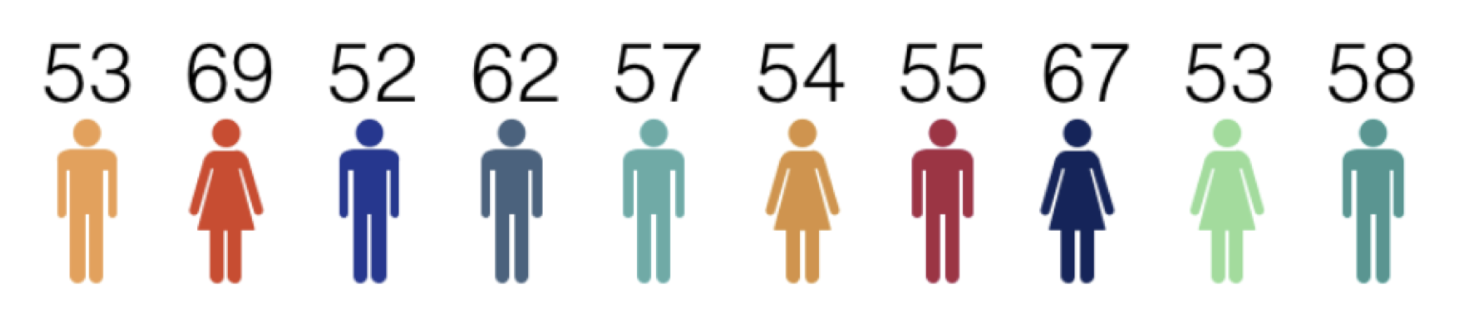
\includegraphics[width=0.4\textwidth,height=\textheight]{img/02Vector.png}

\end{minipage}%

\caption{\label{fig-Help}ตัวอย่างคะแนนสอบวิชาสถิติของนิสิตจำนวน 10 คน}

\end{figure}%

การสร้างเวกเตอร์เพื่อจัดเก็บข้อมูลในโปรแกรม R สามารถทำได้หลายวิธี วิธีการพื้นฐาน
คือการใช้ฟังก์ชัน concatenate \texttt{c()}
เพื่อต่อเชื่อมข้อมูลหลายค่าเข้าด้วยกันให้อยู่ในรูปแบบของ เวกเตอร์ จากนั้นใช้ฟังก์ชัน
\texttt{\textless{}-} เพื่อสร้างตัวแปรสำหรับจัดเก็บเวกเตอร์ที่สร้างขึ้นในข้างต้น
ยกตัวอย่างเช่น ต้องการเก็บข้อมูลคะแนนสอบวิชาสถิติของนิสิตจำนวน 10 คน ดังรูป 2.3
ไว้ในตัวแปรแบบเวกเตอร์ของภาษา R และตั้งชื่อว่า \texttt{score}
สามารถเขียนคำสั่งได้ดังนี้

\begin{Shaded}
\begin{Highlighting}[]
\DocumentationTok{\#\# create score vector }
\NormalTok{score }\OtherTok{\textless{}{-}} \FunctionTok{c}\NormalTok{(}\DecValTok{53}\NormalTok{,}\DecValTok{69}\NormalTok{,}\DecValTok{52}\NormalTok{,}\DecValTok{62}\NormalTok{,}\DecValTok{57}\NormalTok{,}\DecValTok{54}\NormalTok{,}\DecValTok{55}\NormalTok{,}\DecValTok{67}\NormalTok{,}\DecValTok{53}\NormalTok{,}\DecValTok{58}\NormalTok{)}
\DocumentationTok{\#\# print score}
\NormalTok{score}
\end{Highlighting}
\end{Shaded}

\begin{verbatim}
 [1] 53 69 52 62 57 54 55 67 53 58
\end{verbatim}

ตัวอย่างข้างต้นจะเห็นว่าการพิมพ์ชื่อของเวกเตอร์เป็นการเรียกดูสมาชิกทั้งหมด
ภายในเวกเตอร์นั้นเหมือนกับการเรียกดูตัวแปรสเกลาร์ นอกจากนี้เวกเตอร์มีข้อมูลที่จัดเก็บได้
หลายตัวจึงทำให้สามารถเรียกดูข้อมูลบางส่วนหรือทั้งหมดของเวกเตอร์ก็ได้ ในกรณีที่ต้องการ
เรียกดูสมาชิกเพียงบางส่วนของเวกเตอร์สามารถทำได้โดยใช้ลำดับของสมาชิกที่ต้องการภายในเวกเตอร์นั้นเป็นตัวอ้างอิงสมาชิกที่ต้องการ
รูปแบบของคำสั่งประกอบด้วยชื่อของเวกเตอร์แล้วตามด้วยเครื่องหมาย \texttt{{[}i{]}}
โดยที่ \texttt{i} คือลำดับของสมาชิกที่ต้องการ เช่น จากเวกเตอร์ score
หากต้องการเรียกดูคะแนนสอบของนิสิตคนที่ 3 สามารถเขียนคำสั่งเป็น
\texttt{score{[}3{]}} หรือหากต้องการ เรียกคะแนนสอบวิชาสถิติของนิสิตคนที่ 5, 6,
\ldots, 9 สามารถเขียนคำสั่งเป็น \texttt{score{[}5:9{]}}
ผลลัพธ์ที่ได้จะขึ้นอยู่กับจำนวนสมาชิกที่สอดคล้องกับเงื่อนไขที่กำหนด ดังนี้

\begin{Shaded}
\begin{Highlighting}[]
\DocumentationTok{\#\# filter 3rd element from score}
\NormalTok{score[}\DecValTok{3}\NormalTok{]}
\end{Highlighting}
\end{Shaded}

\begin{verbatim}
[1] 52
\end{verbatim}

\begin{Shaded}
\begin{Highlighting}[]
\DocumentationTok{\#\# filter 5th{-}9th elements from score}
\NormalTok{score[}\DecValTok{5}\SpecialCharTok{:}\DecValTok{9}\NormalTok{]}
\end{Highlighting}
\end{Shaded}

\begin{verbatim}
[1] 57 54 55 67 53
\end{verbatim}

\textbf{หมายเหตุ : } \texttt{:} เป็นตัวดำเนินการหนึ่งในภาษา R
ที่ใช้สร้างลำดับเลขคณิตอย่างง่าย โดย \texttt{a:b}
จะได้ผลลัพธ์เป็นลำดับเลขคณิตที่มีพจน์แรกและพจน์สุดท้ายเป็นเลข \texttt{a} และ
\texttt{b} ตามลำดับ โดยที่สมาชิกที่อยู่ระหว่างตัวเลขทั้งสองมีระยะห่างหรือผลต่างร่วมที่เท่ากับ
1 ทั้งนี้ผลลัพธ์ที่ได้จะอยู่ในสถานะเวกเตอร์ ดังนั้น \texttt{5:9}
ในตัวอย่างข้างต้นจึงหมายถึงการสร้างเวกเตอร์ที่มีสมาชิกเป็น 5, 6, 7, 8 และ 9 ตามลำดับ

\begin{Shaded}
\begin{Highlighting}[]
\DecValTok{5}\SpecialCharTok{:}\DecValTok{9}
\end{Highlighting}
\end{Shaded}

\begin{verbatim}
[1] 5 6 7 8 9
\end{verbatim}

ในกรณีต้องการคัดกรองสมาชิกที่ไม่ได้เรียงกันเป็นลำดับ เช่น
ต้องการคัดกรองให้เหลือเฉพาะคะแนนสอบของนิสิตคนที่ 2, 5, 7 และ 10 จากเวกเตอร์
\texttt{score} ผู้วิเคราะห์สามารถสร้างเวกเตอร์ \texttt{element}
เพื่อระบุตำแหน่งของสมาชิกในเวกเตอร์ \texttt{score} ที่ต้องการเลือก
จากนั้นจึงใช้เวกเตอร์ \texttt{element} เป็นตัวคัดกรอง ดังตัวอย่าง

\begin{Shaded}
\begin{Highlighting}[]
\DocumentationTok{\#\# create element vector}
\NormalTok{element }\OtherTok{\textless{}{-}} \FunctionTok{c}\NormalTok{(}\DecValTok{2}\NormalTok{, }\DecValTok{5}\NormalTok{, }\DecValTok{7}\NormalTok{, }\DecValTok{10}\NormalTok{)}
\DocumentationTok{\#\# using element to filter score}
\NormalTok{score[element]}
\end{Highlighting}
\end{Shaded}

\begin{verbatim}
[1] 69 57 55 58
\end{verbatim}

การอ้างอิง/คัดกรองสมาชิกภายในเวกเตอร์ข้างต้น
สามารถนำมาใช้เพื่อแก้ไขหรือเปลี่ยนแปลงค่าของสมาชิกภายในเวกเตอร์ได้อีกด้วย
โดยใช้งานร่วมกับตัวดำเนินการ \texttt{\textless{}-} ยกตัวอย่างเช่น
หากพบว่าในเวกเตอร์ \texttt{score} มีการบันทึกคะแนนสอบของนิสิตคนที่ 6 คลาดเคลื่อนไป
โดยที่ถูกต้องจะต้องมีค่าเท่ากับ 60 คะแนน สามารถดำเนินการแก้ไขและบันทึกค่าใหม่ได้ดังนี้

\begin{Shaded}
\begin{Highlighting}[]
\DocumentationTok{\#\# assign new value to 6th element of score}
\NormalTok{score[}\DecValTok{6}\NormalTok{] }\OtherTok{\textless{}{-}} \DecValTok{60}
\DocumentationTok{\#\# print score}
\NormalTok{score}
\end{Highlighting}
\end{Shaded}

\begin{verbatim}
 [1] 53 69 52 62 57 60 55 67 53 58
\end{verbatim}

ในทำนองเดียวกับตัวแปรสเกลาร์ เราอาจจำแนกเวกเตอร์ได้เป็น 3 ประเภท ได้แก่
เวกเตอร์ตัวเลข (numeric vectors) เวกเตอร์ตัวอักษร (character vectors)
และเวกเตอร์ตรรกะ (logical vectors) ทั้งนี้การสร้างเวกเตอร์ทั้ง 2
ประเภทที่เหลือมีลักษณะที่เป็นไปในหลักเดียวกับการสร้างตัวแปรตัวอักษร และตรรกะ
กล่าวคือการสร้างเวกเตอร์ตัวอักษรสามารถทำได้โดยใช้ตัวดำเนินการ
\texttt{\textless{}-} ร่วมกับ \texttt{c()} เหมือนเดิม
แต่สมาชิกแต่ละตัวที่เป็นข้อความหรือตัวอักษรจะต้องถูกระบุไว้ภายใต้เครื่องหมาย quotation
(\texttt{"\ "}) ในทำนองเดียวกับการสร้างตัวแปรตัวอักษร ดังตัวอย่าง

\begin{Shaded}
\begin{Highlighting}[]
\DocumentationTok{\#\# create gender vector}
\NormalTok{gender }\OtherTok{\textless{}{-}} \FunctionTok{c}\NormalTok{(}\StringTok{"M"}\NormalTok{,}\StringTok{"F"}\NormalTok{,}\StringTok{"M"}\NormalTok{,}\StringTok{"M"}\NormalTok{,}\StringTok{"M"}\NormalTok{,}\StringTok{"F"}\NormalTok{,}\StringTok{"M"}\NormalTok{,}\StringTok{"F"}\NormalTok{,}\StringTok{"F"}\NormalTok{,}\StringTok{"M"}\NormalTok{)}
\DocumentationTok{\#\# print gender}
\end{Highlighting}
\end{Shaded}

\bookmarksetup{startatroot}

\chapter{Summary}\label{summary}

In summary, this book has no content whatsoever.

\begin{Shaded}
\begin{Highlighting}[]
\DecValTok{1} \SpecialCharTok{+} \DecValTok{1}
\end{Highlighting}
\end{Shaded}

\begin{verbatim}
[1] 2
\end{verbatim}

\bookmarksetup{startatroot}

\chapter*{References}\label{references}
\addcontentsline{toc}{chapter}{References}

\markboth{References}{References}

\phantomsection\label{refs}
\begin{CSLReferences}{0}{1}
\end{CSLReferences}


\backmatter


\end{document}
